\documentclass[
	openany,
	10pt,
	parindent=0
] {article}

\usepackage[a5paper,top=2cm,bottom=2cm,left=1.5cm,right=1.5cm]{geometry}

\usepackage{import}
\usepackage[T2A]{fontenc}
\usepackage[english,russian]{babel}

\usepackage{amsmath}
\usepackage{amsfonts}
\usepackage{amssymb}
\usepackage{amsthm}

\usepackage{braket}
\usepackage{blkarray}
\usepackage{graphics}
\usepackage{graphicx}
\usepackage{subcaption}

\usepackage{titlesec}
\usepackage{enumitem}
\usepackage{parskip}
\usepackage{setspace}
\usepackage{multicol}

\setstretch{1}
\setlength{\parindent}{0pt}
\graphicspath{{images/}}

\usepackage{tikz}
	\usetikzlibrary{arrows.meta}
	\usetikzlibrary{graphs, graphs.standard}

\tikzset{
	node distance={12mm}, minimum size={5mm}, inner sep={0mm}, main/.style = {draw, circle}
}

\titleformat{\section}[block]{\normalfont\bfseries\normalsize}{\thesection}{0.3em}{}
\titlespacing*{\section}{0em}{0pt}{10pt}

\newtheoremstyle{custom} % Имя стиля
  {3pt}      % Отступ сверху
  {3pt}      % Отступ снизу
  {\normalsize} % Шрифт для тела теоремы
  {}         % Величина отступа
  {\bfseries}% Шрифт заголовка теоремы
  {}         % Знак препинания после заголовка теоремы
  { }        % Пробел после заголовка теоремы
  {\thmname{#1}\thmnote{ \bfseries#3}} % Спецификация заголовка теоремы

\theoremstyle{custom}
\newtheorem{theorem}{Теорема:}[section]
\newtheorem{definition}{Опр:}[section]
\makeatletter
\renewenvironment{proof}[1][\proofname]{\par
  \pushQED{\qed}%
  \normalfont \topsep6\p@\@plus6\p@\relax
  \trivlist
  \item[\hskip\labelsep
        \bfseries
    Док-во:\@addpunct{}]%
    \ignorespaces
}{%
  \popQED\endtrivlist\@endpefalse
}
\makeatother


\newcommand*{\titleASU}{\begingroup
	\begin{center}
        \large
		Санкт-Петербургский государственный электротехнический университет
		имени В. И. Ленина "ЛЭТИ"
		\vfill
		билеты \\ 
		\huge{\textbf{КОМБИНАТОРИКА И ТЕОРИЯ ГРАФОВ}} \\
        \vspace*{200pt}
        \large
        Студент: \hfill Придчин В.Е.\\
        Группа: \hfill 2308 \\
        Лектор: \hfill Зяблицева Л.
		\vfill
    \LaTeX
    \vfill
		Санкт-Петербург \\ 2024
		\newpage
	\end{center}
\endgroup}

\begin{document}
  \begin{titlepage}
      \titleASU
  \end{titlepage}

  \setcounter{page}{2}

  \section{Основные определения теории графов. Смежность и инцидентность вершин и ребер графа. 
Степени вершин в графе и орграфе. Теоремы о сумме степеней вершин в графе и орграфе. 
Матрицы смежности и инцидентности. Найти матрицы смежности и инцидентности указанного 
графа.}

$V$ -- множество вершин. \\
$E$ -- множество пар вида $(u, v): u, v \in V$ (множество ребер).

\begin{definition}
    Графом -- называют совокупность 2-ух множеств непустого множества E
	\begin{equation*}
		E = \{(u, v): u, v \in V\}, \; G(V, E) - \textit{обозначение графа}
	\end{equation*}
\end{definition}

\begin{definition}
    Петля -- пара вида $(v,v)$ в множестве $E$.
\end{definition}

\begin{definition}
    Кратные ребра -- одинаковые пары в множестве $E$. Количество кратных ребер - кратность ребра.
\end{definition}

\noindent
Существуют следующие виды графов:
\begin{enumerate}[left=0.0em, labelsep=1em, topsep=0.5em, itemsep=0pt, parsep=0.5em]
    \item Псевдограф -- в графе могут быть и \textit{кратные ребра}, и \textit{петли}.
    \item Мультиграф -- в графе есть \textit{кратные ребра}, но нет \textit{петель}.
    \item Простой граф -- отсутствуют и \textit{кратные ребра} и \textit{петли}.
\end{enumerate}

\begin{definition}
    Ориентированный граф (орграф) -- граф с ориентированными ребрами.
\end{definition}

\begin{definition}
    Если $e=(u,v)$ -- ребро неориентированного графа, то $u, v$ - концы ребра.
\end{definition}

\begin{definition}
    Если $e=(u,v)$ -- ребро (дуга) ориентированного графа, то $u$ - начало ребра, $v$ - конец ребра.
\end{definition}

\begin{definition}
    $a, b \text{ \textit{смежные}} \Leftrightarrow e=(u,v)$.
\end{definition}

\begin{definition}
    $u, v \text{ \textit{инцидентны ребру }} e \Leftrightarrow e=(u,v)$.
\end{definition}

\begin{definition}
	Степенью вершины $v$ неориентированного графа называется количество ребер инцидентных данной вершине, $\delta(v)$ (петлю считают два \mbox{раза}).
\end{definition}

\begin{minipage}{0.55\textwidth}
	\centering
	\begin{tikzpicture}
		\node[main] (1) {$1$};
		\node[main] (3) [above right of=1] {$3$};
		\node[main] (5) [below right of=3] {$5$};
		\node[main] (2) [above of=5] {$2$};
		\node[main] (4) [below left of=5] {$4$};
		
		\draw (3) to [out=90,in=180,looseness=5] (3);
		\draw (1) -- (3);
		\draw (3) -- (5);
		\draw (1) -- (5);
		\draw (4) -- (5);
	\end{tikzpicture}
\end{minipage}
\begin{minipage}{0.3\textwidth}
	$\begin{aligned}
		&\delta(1) = 2 & \delta(4) &= 1 \\
		&\delta(2) = 0 & \delta(5) &= 3 \\
		&\delta(3) = 4 & \Rightarrow sum &= 10
	\end{aligned}$
\end{minipage}

\begin{theorem}
    Сумма степеней вершин неориентированного графа равна удвоенному числу ребер
	\begin{align*}
		\sum_{u \in V}\delta(v)=2r, \textit{ где r - число ребер}
	\end{align*}
\end{theorem}

\begin{proof}
    Теорема справедлива, так как вклад каждого ребра равен двум.
\end{proof}

\begin{definition}
    Если степень вершины равна нулю, то вершина \textit{изолированная}, \\ $\delta(v)=0$.
\end{definition}

\begin{definition}
    Если степень вершины равна единице, то вершина \textit{висячая}, $\delta(v)=1$
\end{definition}

\begin{definition}
    Полустепенью исхода(захода) вершина $v$ ориентированного графа называют количество ребер исходящих(заходящих) в данную вершину.
    \begin{tikzpicture}[baseline={(A.base)}]
		\node [text width=5cm] (A) at (0,0) {$\delta^-(v)$ -- полустепень исхода\\
			$\delta^+(v)$ -- полустепень захода};
	\end{tikzpicture}
\end{definition}

\begin{theorem}
	Для орграфа справедливо равенство
	\begin{align*}
		\sum_{u \in V}\delta^-(v)=\sum_{u \in V}\delta^+(v)=r, \textit{ где r -- число ребер}
	\end{align*}
\end{theorem}

\begin{minipage}{0.5\textwidth}
	\centering
	\begin{tikzpicture}
		\node[main] (a) {$a$};
		\node[main] (d) [right of=a] {$d$};
		\node[main] (b) [above of=d] {$b$};
		\node[main] (c) [right of=b] {$c$};
		\node[main] (e) [below of=d] {$e$};
		
		\draw[-{Stealth[length=2mm]}] (e) to [out=270,in=360,looseness=5] (e);
		\draw[-{Stealth[length=2mm]}] (a) -- (d);
		\draw[-{Stealth[length=2mm]}] (a) -- (e);
		\draw[-{Stealth[length=2mm]}] (a) -- (b);
		\draw[-{Stealth[length=2mm]}] (b) -- (c);
		\draw[-{Stealth[length=2mm]}] (e) -- (d);
	\end{tikzpicture}
\end{minipage}
\begin{minipage}{0.5\textwidth}
	$\begin{aligned}
		\delta^-(a) &= 3 &\delta^+(a) = 0 \\
		\delta^-(b) &= 1 &\delta^+(b) = 1 \\
		\delta^-(c) &= 0 &\delta^+(c) = 1 \\
		\delta^-(d) &= 0 &\delta^+(d) = 2 \\
		\delta^-(e) &= 2 &\delta^+(e) = 2 \\
		\sum\delta^-(v) &= 6; \; &\sum\delta^+(v) = 6 \\
	\end{aligned}$
\end{minipage}

\begin{definition}
    Матрицей смежности графа(орграфа) называют квадратную матрицу размерностью $n$, где $n=|v|$ (мощность множества вершин), в котором $a_{ij}=k$, где $k$ - число ребер $(v_i,v_j)$
\end{definition}

\begin{definition}
    Пусть $G(V,E)$ -- неориентированный граф. Матрицей инцидентности неориентированного графа называется матрица $B$ размером $n*r$, $|v| = n, |E| = r$, где каждый элемент матрицы:
	\begin{align*}
		b_{ij}=\left\{\begin{array}{l}
			1, \text{ если $v_i$ инцидентно ребру $e_j$}
			\\ 
			0, \text{ иначе}
		\end{array}\right.
	\end{align*}
\end{definition}
\noindent
Такая матрица будет симметричной.

\begin{definition}
    Пусть $G(V,E)$ -- ориентированный граф. Матрицей инцидентности ориентированного графа называется матрица $B$ размером $n*r$, $|v| = n, |E| = r$, где каждый элемент матрицы:
	\begin{align*}
		b_{ij}=\left\{\begin{array}{l}
			-1, \text{ если ребро $e_j$ выходит из $v_i$}
			\\
			1, \text{ если ребро $e_j$ входит из $v_i$}
			\\ 
			0, \text{ иначе}
		\end{array}\right.
	\end{align*}
\end{definition}

Если есть петля, то на соответствующее место ставят любое число.

Поиск матрицы смежности $A$ и инцидентности $B$ для неориентированного графа:
\begin{figure}[ht]
	\centering
	\begin{minipage}[b]{0.45\linewidth}
		\centering
		\begin{tikzpicture}[node distance=30mm]
			\node[main] (a) {$a$};
			\node[main] (b) [above of=a] {$b$};
			\node[main] (c) [right of=b] {$c$};
			\node[main] (d) [below of=c] {$d$};
			
			\draw[] (a) -- node[midway, left]{$e_1$} (b);
			\draw[] (a) -- node[midway, below right]{$e_2$} (c);
			\draw[] (b) to [out=30, in= 150] node[midway, above]{$e_3$} (c);
			\draw[] (b) -- node[midway, below]{$e_4$} (c);
			\draw[] (c) -- node[midway, right]{$e_5$} (d);
			\draw[] (d) to [out=270,in=360,looseness=5] node[midway, below right]{$e_6$} (d);
		\end{tikzpicture}
	\end{minipage}
	\begin{minipage}[b]{0.45\linewidth}
		\begin{flalign*}
			&A =
			\begin{blockarray}{ccccc}
				& a & b & c & d \\
				\begin{block}{c(cccc)}
					a & 0 & 1 & 1 & 0 \\
					b & 1 & 0 & 2 & 0 \\
					c & 1 & 2 & 0 & 1 \\
					d & 0 & 0 & 1 & 1 \\
				\end{block}
			\end{blockarray} \\
			&B =
			\begin{blockarray}{ccccccc}
				& e_1 & e_2 & e_3 & e_4 & e_5 & e_6 \\
				\begin{block}{c(cccccc)}
					a & 1 & 1 & 0 & 0 & 0 & 0\\
					b & 1 & 0 & 1 & 1 & 0 & 0\\
					c & 0 & 1 & 1 & 1 & 1 & 0\\
					d & 0 & 0 & 0 & 0 & 1 & 1\\
				\end{block}
			\end{blockarray}
		\end{flalign*}
	\end{minipage}
\end{figure}

\newpage
Поиск матрицы смежности $A$ и инцидентности $B$ для ориентированного графа:
\begin{figure}[ht]
	\centering
	\begin{minipage}[b]{0.40\linewidth}
		\begin{tikzpicture}[node distance=22mm, minimum size=17, remember picture, overlay]
			\node[main] (a) at ([xshift=-5.2cm, yshift=5cm]current page) {$a$};
			\node[main] (b) [above right of=a] {$b$};
			\node[main] (c) [right of=b] {$c$};
			\node[main] (d) [right of=a] {$d$};
			\node[main] (e) [below right of=a] {$e$};
			
			\draw[-{Stealth[length=2mm]}] (e) to [out=270,in=360,looseness=5] node[midway, below]{$e_6$}(e);
			\draw[-{Stealth[length=2mm]}] (a) -- node[midway, above]{$e_2$} (d);
			\draw[-{Stealth[length=2mm]}] (a) -- node[midway, below left]{$e_3$} (e);
			\draw[-{Stealth[length=2mm]}] (a) -- node[midway, left]{$e_1$} (b);
			\draw[-{Stealth[length=2mm]}] (b) -- node[midway, below]{$e_4$} (c);
			\draw[-{Stealth[length=2mm]}] (e) -- node[midway, left]{$e_5$} (d);
		\end{tikzpicture}
		\hfil
	\end{minipage}
	\begin{minipage}[t]{0.45\linewidth}
		\vspace*{-5mm}
		\begin{flalign*}
			&A =
			\begin{blockarray}{cccccc}
				& a & b & c & d & e\\
				\begin{block}{c(ccccc)}
					a & 0 & 1 & 0 & 1 & 1 \\
					b & 0 & 0 & 1 & 0 & 0 \\
					c & 0 & 0 & 0 & 0 & 0 \\
					d & 0 & 0 & 0 & 0 & 0 \\
					e & 0 & 0 & 0 & 1 & 1 \\
				\end{block}
			\end{blockarray} \\
			&B =
			\begin{blockarray}{ccccccc}
				& e_1 & e_2 & e_3 & e_4 & e_5 & e_6 \\
				\begin{block}{c(cccccc)}
					a & -1 & -1 & -1 & 0 & 0 & 0\\
					b & 1 & 0 & 0 & -1 & 0 & 0\\
					c & 0 & 0 & 0 & 1 & 0 & 0\\
					d & 0 & 1 & 0 & 0 & 1 & 0\\
					e & 0 & 0 & 1 & 0 & -1 & 1\\
				\end{block}
			\end{blockarray}
		\end{flalign*}
	\end{minipage}
\end{figure}
	\section{Полные и двудольные графы. Число ребер в полном графе с n вершинами и в полном 
двудольном графе (вывод формул).}

\begin{definition}
    \textit{Полный граф} -- простой неориентированный граф у которого любые две вершины смежны.
\end{definition}

\begin{tikzpicture}
    % K1
    \graph[nodes={draw, circle}] { subgraph K_n [n=1,clockwise,radius=0.8mm] };
    \node at (0,-1.5) {$K_1$};
  
    % K2
    \begin{scope}[xshift=6.5em]
        \graph[nodes={draw, circle}] { subgraph K_n [n=2,clockwise,radius=0.8cm] };
      \node at (0,-1.5) {$K_2$};
    \end{scope}
  
    % K3
    \begin{scope}[xshift=14em]
        \graph[nodes={draw, circle}] { subgraph K_n [n=3,clockwise,radius=0.8cm] };
      \node at (0,-1.5) {$K_3$};
    \end{scope}
  
    % K4
    \begin{scope}[xshift=22em]
        \graph[nodes={draw, circle}] { subgraph K_n [n=4,clockwise,radius=0.8cm] };
      \node at (0,-1.5) {$K_4$};
    \end{scope}
  
    % K5
    \begin{scope}[xshift=30em]
        \graph[nodes={draw, circle}] { subgraph K_n [n=5,clockwise,radius=0.8cm] };
      \node at (0,-1.5) {$K_5$};
    \end{scope}
  \end{tikzpicture}

Количество полных ребер в графе $K_n = C_n^2= \frac{n!}{2!(n-2)!} = \frac{n(n-1)}{2}$.

\begin{definition}
    \textit{Двудольный граф} -- граф, если его множество вершин $V$ можно разделить на подмножество $V_1$ и $V_2$ такое что:
	\begin{tikzpicture}[baseline={(A.base)}]
		\node [text width=2cm] (A) at (0,0) {$V_1 \cap V_2 = \varnothing$\\
			$V_1 \cup V_2 = V$};
	\end{tikzpicture}
\end{definition}

Смежными могут быть только вершины из разных долей графа.

\begin{center}
\begin{tikzpicture}
	\graph[nodes={draw, circle}] {
		subgraph I_nm [V={1, 2, 3}, W={4, 5}];
		
		1 -- { 4, 5};
		2 -- { 4, 5};
		3 -- { 5 }
	};

    \node[anchor=west] at (2, -0.5) {
        \begin{minipage}{4cm}
        \begin{align*}
            V &= \{1, 2, 3, 4, 5\} \\
            V_1 &= \{1, 2, 3\} \\
            V_2 &= \{4, 5\}
        \end{align*}
        \end{minipage}
    };
\end{tikzpicture}
\end{center}

\begin{definition}
    \textit{Полный двудольный граф} -- каждая вершина одной доли соединяется с другой.
    $K_{t_1, k_2}$, где ${t_1, k_2}$ -- количество вершин в долях графа.
\end{definition}

\begin{center}
\begin{tikzpicture}
	\graph[nodes={draw, circle}] {
		subgraph I_nm [V={1, 2, 3}, W={4, 5, 6}];
		
		1 -- { 4, 5, 6};
		2 -- { 4, 5, 6};
		3 -- { 4, 5, 6}
	};

    \node[anchor=west] at (2, -0.5) {
        \begin{minipage}{4cm}
        \begin{align*}
            K_{3,3}\\
            V &= \{1, 2, 3, 4, 5, 6\} \\
            V_1 &= \{1, 2, 3\} \\
            V_2 &= \{4, 5, 6\}
        \end{align*}
        \end{minipage}
    };
\end{tikzpicture}
\end{center}

В полном двудольном графе содержится $t_1 \cdot t_2$ ребер.
	\section{Изоморфизм и гомеоморфизм графов. Примеры изоморфных и гомеоморфных графов. Способы 
проверки изоморфизма графов. Инварианты графа. Дополнение графа, проверка изоморфизма 
графов с помощью дополнений. Выяснить, являются ли графы G1 и G2 изоморфными, 
гомеоморфными.}

\begin{definition}
    \textit{Изоморфизм графов} -- биективное отображение $\varphi: V_1 \rightarrow V_2$, такое что:
    \begin{align*}
        (\forall u,v \in V)((u,v) \in E_1) \Leftrightarrow (\varphi(u),\varphi(v)) \in E_2
    \end{align*}
\end{definition}

Изоморфные графы обозначаются: $G_1 \cong G_2$

Изоморфные объекты \textit{не различимы} с точки зрения математики. Это экземпляры
одного и того же математического объекта. Изоморфные объекты имеют одинаковое
число элементов и свойств.

Изоморфизм графов можно определить:
\begin{enumerate}[left=0.0em, labelsep=1em, topsep=0.0em, itemsep=0pt, parsep=0.5em]
    \item По определению (найдя биективное отображение множества вершин,
    сохраняющее смежность)
    \item Перерисовав один из графов так, чтобы изображение совпало с другим
    графом
    \item Сравнив матрицы смежности графов
\end{enumerate}

\begin{theorem}
    Графы изоморфны тогда и только тогда, когда матрицу смежности
одного из них можно получить из матрицы смежности другого путём
одновременной перестановки местами $i$-ой и $j$-ой строк и столбцов.
\end{theorem}

Пример изоморфных графов:
\begin{figure}[h]
    \centering
    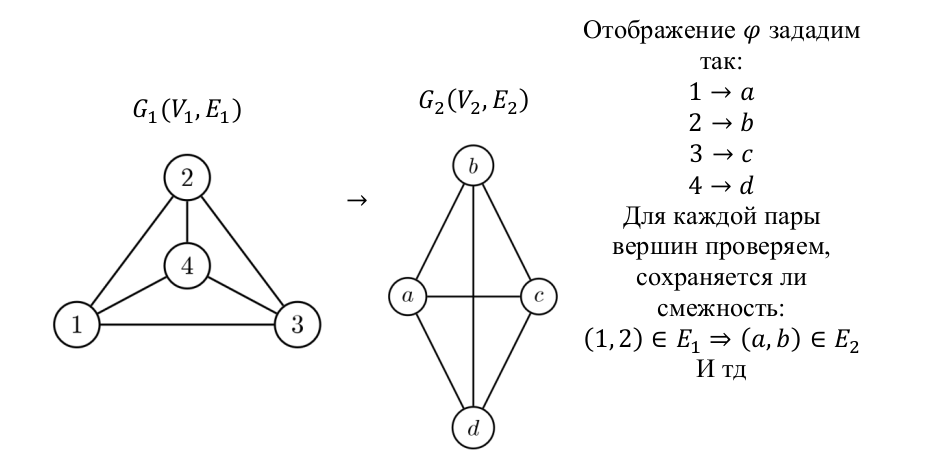
\includegraphics[scale=0.25]{3_iso.png}
\end{figure}

\begin{definition}
    \textit{Инвариантом изоморфизма графов} называется некоторое
    (обычно числовое) значение или упорядоченный набор значений,
    характеризующий структуру графа и не зависящий от способа его задания.
\end{definition}

Инвариантами графа являются:
\begin{enumerate}[left=0.0em, labelsep=1em, topsep=0.0em, itemsep=0pt, parsep=0.5em]
    \item Количество вершин
    \item Количество ребер
    \item Набор степеней вершин (упорядоченный)
    \item Определитель матрицы смежности
    \item Количество компонент связности
    \item Хроматическое число и т.д.
\end{enumerate}

Пусть $G(V,E)$ -- простой неориентированный граф.

\begin{definition}
    Дополнением графа $G$ называется граф $\overline{G}(\overline{V},\overline{E})$,
    у которого $\overline{V}=V$, в множестве $\overline{E}$ содержатся ребра полного графа,
    которых нет в множестве $E$.
\end{definition}

\begin{theorem}
    Простые графы $G$ и $H$ изоморфны тогда и только тогда, когда изоморфны их дополнения.
    \begin{align*}
        G \cong H \Leftrightarrow \overline{G} \cong \overline{H}
    \end{align*}
\end{theorem}

\begin{definition}
    Граф является самодополнительным, если он изоморфен своему дополнению.
\end{definition}

Понятие изоморфизма можно дать и для произвольных графов.

\begin{definition}
    Граф $G_1(V_1,E_1)$ и $G_2(V_2,E_2)$ \textit{изоморфны}, если $\exists$
    биективные отображения $\varphi : V_1 \rightarrow V_2$ и $h: E_1 \rightarrow E_2$
    такие, что:
    $$e = (u,v) \in E_1 \Leftrightarrow h(e) = (\varphi(u),\varphi(v)) \in E_2$$
\end{definition}

\newpage
\textbf{Гомеоморфизм графов}

\begin{definition}
    \textit{Операция подразбиения ребра} $(u, v)$ состоит в удалении этого
    ребра, добавлении вершины $\omega$ и рёбер $(u, \omega)$ и $(\omega, v)$.
\end{definition}

\begin{definition}
    Граф $G_2$ называется \textit{подразбиением} графа $G_1$, если его можно
    получить из графа $G_1$ путём последовательного применения операции
    подразбиения рёбер (сам граф тоже является своим подразбиением).
\end{definition}

\begin{figure}[h]
    \centering
    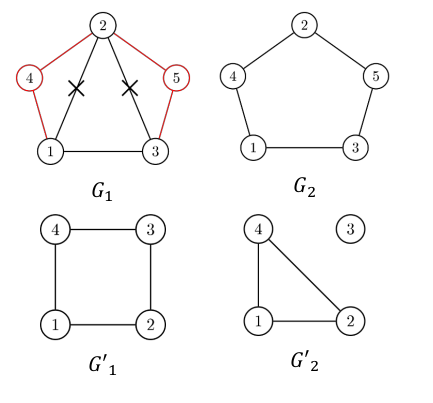
\includegraphics[scale=0.4]{3_2.png}
\end{figure}

Графы $G_1$ и $G_2$ на рисунке гомеоморфны, потому что их подразбиения
изоморфны.

Покажем, что графы ${G_1}'$ и ${G_2}'$ не гомеоморфны.

При любой операции подразбиения ребер появляются вершины степени 2, у
остальных вершин степень не меняется. В графе ${G_2}'$ есть вершина степени 0,
она останется такой при любом количестве операций подразбиения ребер. В
графе ${G_1}'$ все вершины имеют степень 2. При любом количестве операций
подразбиения ребер появятся вершины степени 2, у имеющихся вершин
степень не изменится. Это значит, что любые подразбиения графов не
являются изоморфными, поэтому графы ${G_1}'$ и ${G_2}'$ на рисунке не
гомеоморфны.
	\section{Маршруты, цепи, циклы в графе. Метрические характеристики графа. Найти эксцентриситет 
вершины указанного графа, радиус, диаметр графа, центральные и периферийные вершины 
указанного графа.}
	\section{Алгоритмы обхода графа в глубину и ширину.}

\begin{definition}
    Обход графа (поиск на графе) –- это процесс систематического просмотра
    всех ребер или вершин графа с целью отыскания ребер или вершин,
    удовлетворяющих некоторому условию.
\end{definition}

\begin{definition}
    Поиск в ширину (BFS) нужен для нахождения расстояний между вершин в связном графе.
    Алгоритм по принципу напоминает "пожар".
\end{definition}

Алгоритм поиска в ширину:
\begin{enumerate}[left=0.0em, labelsep=1em, topsep=0em, itemsep=0pt, parsep=0.5em]
    \item Все вершины окрашиваются в белый цвет.
    \item Выбирается первая вершина, раскрашивается в черный цвет и заносится в очередь.
    \item Посещается первая вершина из очереди. Все смежные с ней белые вершины
    раскрашиваются в черный цвет и заносятся в очередь. После этого эта вершина удаляется
    из очереди.
    \item Повторяется шаг 3 до тех пор пока очередь не пуста.
\end{enumerate}

\begin{figure}[h]
    \centering
    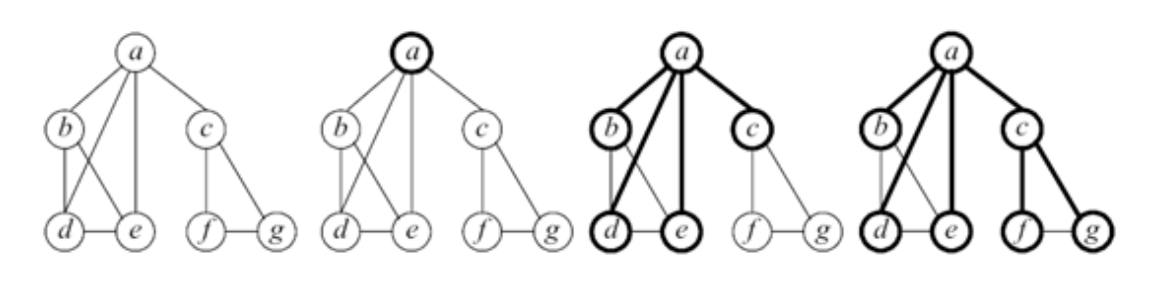
\includegraphics[width=\textwidth]{5_bfs.png}
\end{figure}

Сложность поиска в ширину при нематричном представлении графа
равна $O(n+m)$, так как рассматриваются все n вершин и m ребер.
Использование матрицы смежности приводит к оценке $O(n^2)$.

Если граф не является связным, то нужно добавить шаг 5, в
котором написать, что нужно повторять 2 шаг до тех пор, пока в графе не
останется белых вершин.

Если сначала присвоить первой вершине значение 0, потом
смежным с ней вершинам 0+1 =1, и так далее, то в итоге для каждой
вершины будет найдено расстояние от первой вершины.
\newpage

\begin{definition}
    Поиск в глубину (DFS) исследует конкретную ветку в графе и только потом переходит к другой (если они остануться нерассмотренными).
\end{definition}

Вершины графа могут быть раскрашены в три цвета: белый цвет означает, что
в вершине еще не были, серый – что в вершине были, но еще вернемся, черный
– что были и больше не рассматриваем.

Алгоритм поиска в глубину:
\begin{enumerate}[left=0.0em, labelsep=1em, topsep=0em, itemsep=0pt, parsep=0.5em]
    \item Всем вершинам графа присваиваем белый цвет.
    \item Выбираем первую вершину и раскрашиваем в серый цвет.
    \item Для последней раскрашенной в серый цвет вершины выбираем белую
    смежную ей вершину (если такая вершина есть), раскрашиваем ее в серый цвет
    и переходим к шагу 3.
    \item Повторяем шаг 3 до тех пор, пока все вершины не будут раскрашены в
    черный цвет.
\end{enumerate}

Если для рассматриваемой вершины белых смежных с ней вершин нет, то
рассматриваемую вершину раскрашиваем в черный цвет и переходим к шагу
3.

\begin{figure}[h]
    \centering
    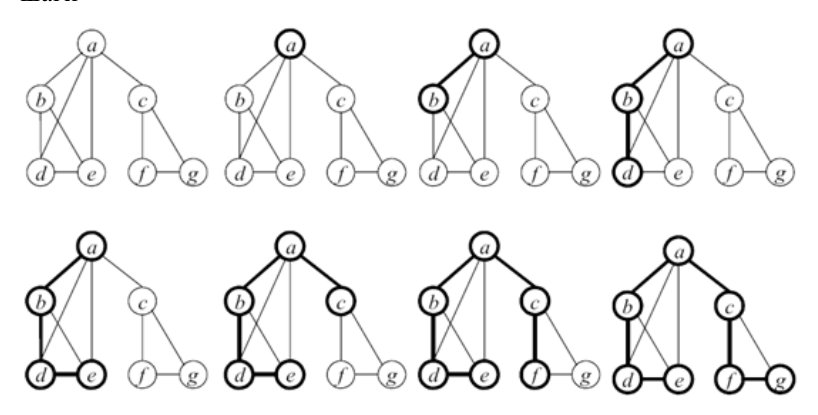
\includegraphics[width=\textwidth]{5_dfs.png}
\end{figure}

Временная сложность алгоритма зависит от представления графа. Если
применена матрица смежности, то временная сложность равна $O(n^2)$, а если
нематричное представление -- $O(n+m)$: рассматриваются все вершины и все ребра.
  \section{Прямое произведение множеств, мощность прямого произведения конечных множеств. 
Бинарные отношения между множествами A и B. Граф бинарного отношения Матрица 
бинарного отношения, область определения и значений бинарного отношения. Отношение, 
обратное к данному отношению. Найти отношение, изобразить его граф, найти матрицу.}

Пусть $A$ и $B$ -- не пустые множества.
\begin{definition}
    \textit{Прямым (декартовым) произведением множеств $A$ и $B$}
    называют множество всевозможных упорядоченных пар $(a, b), a \in A, b \in B$.
    \begin{align*}
        A \times B = \set{(a,b) | a \in A, b \in B}
    \end{align*}
\end{definition}

Пример:
\begin{align*}
    A &= \set{1,2}, B=\set{a,b,c} \\
    A \times B &= \set{(1, a) , (1, b), (1, c), (2, a), (2, b), (2, c)} \\
    |A| &= n, |B| = m, |A \times B| = n \cdot m
\end{align*}

Если $A=B$, то пишут $A \times A = A^2$.

\begin{definition}
    \textit{Кортеж длины s} -- упорядоченный набор $(a_1,a_2,\dots,a_s)$, где $a \in A_i$.
    \begin{align*}
        A_1 \times A_2 \times \dots \times A_s = \set{(a_1,a_2,\dots,a_s), a_i \in A_i, i \in \overline{1,s}} \\
        |A_i| = t_i \\
        \text{Тогда: } |A_1 \times A_2 \times \dots \times A_s| = t_1 \cdot t_2 \cdot \dots \cdot t_s \\
        \text{Если: } A_1=A_2=\cdots=A_s=A, \text{ то пишут } A_1 \times A_2 \times \dots \times A_s = A^s
    \end{align*}
\end{definition}

\begin{definition}
    \textit{Бинарным отношение между множествами $A$ и $B$} называется
    любое подмножество их прямого произведения.
    Бинарные отношение принято записывать большими буквами или малыми буквами:
    \begin{align*}
        A&=\set{1,2},B=\set{a,b,c}\\
        R&=\set{(1,a),(2,b),(2,c)}\\
        f&=\set{(1,b),(2,a)}
    \end{align*}
    Если $(a,b) \in R$, то говорят, что элементы $a$ и $b$ связаные отношение $R$
    или находятся в отношении $R$. Обозначают: $aRb$.
\end{definition}

Сам граф бинарного отношения будет иметь вид:
\begin{figure}[h]
    \centering
    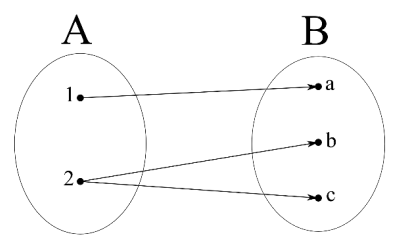
\includegraphics[scale=0.5]{6_grapg.png}
\end{figure}

Пусть бинарное отношение $R \subset A \times B, |A|=n, |B|=m$.
\begin{definition}
    \textit{Матрицой бинарного отношения R} называется матрица \mbox{$C(R) \in M_{n \times m}$},
    элементы которой находятся по правилу:
    \begin{align*}
        c_{ij}=\begin{cases}
        1, \text{ если } a_iRb_j \\
        0, \text{ иначе} 
        \end{cases}.
    \end{align*}
    Пример:
    \begin{align*}
        A&=\set{1,2}, B=\set{a,b,c} \\
        R&=\set{(1,a),(2,b),(2,c)} \\
        C(R)&=\begin{pmatrix}
            1 & 0 & 0 \\
            0 & 1 & 1
        \end{pmatrix}
    \end{align*}
\end{definition}

\begin{definition}
    \textit{Областью определения бинарного отношения $R$} называется
    множество первых элементов пар бинарного отношения.
    \begin{align*}
        D(R)=\set{x \in A | (\exists y \in B)(xRy)}
    \end{align*}
\end{definition}

\begin{definition}
    \textit{Областью значений бинарного отношения $R$} называется
    множество вторых элементов пар бинарного отношения.
    \begin{align*}
        E(R)=\set{y \in B | (\exists x \in A)(xRy)}
    \end{align*}
\end{definition}

Пример:
\begin{align*}
    A&=\set{1,2}, \; B=\set{a,b,c} \\
    R&=\set{(1,b),(2,c),(2,a),(2,b)} \\
    D(R)&=\set{1,2}, \; E(R)=\set{a,b,c}
\end{align*}

\begin{definition}
    \textit{Обратное бинарное отношение к $R$ ($R^{-1}$)} называется им,
    если: $$R^{-1}=\set{(y,x)|(x,y) \in R}$$
\end{definition}

Пример:
\begin{align*}
    R&=\set{(1,b),(2,c),(2,a),(2,b)} \\
    C(R)&=\begin{pmatrix}
        0 & 1 & 0 \\
        1 & 1 & 1
        \end{pmatrix} \\
    R^{-1}&=\set{(b,1),(c,2),(a,2),(b,2)} \\
    C(R)&=\begin{pmatrix}
        0 & 1 \\
        1 & 1 \\
        0 & 1
        \end{pmatrix}
\end{align*}
{
Заметим, что матрица $C(R^{-1})$ является транспонированной
матрицей $C(R)$.
  \section{Свойства бинарных отношений: рефлексивность, антирефлексивность, симметричность, 
антисимметричность, асимметричность, транзитивность. Свойства матриц и графов таких 
отношений, число таких отношений, заданных на n-элементном множестве.}

Будем рассматривать бинарные отношения на множестве $A^2$ в этом случае говорят что бинарное отношение задано на множестве $A$.

\begin{definition}
	Бинарное отношение $R$, заданное на множестве $A$ называется \textit{рефлексивным}, если для любого $a \in A$ верно $aRa$.
	\begin{align*}
		R - \textit{рефлексивно} \iff (\forall a \in A) \; aRa
	\end{align*}
	Если $R$ рефлексивное отношение, то квадратная матрица размера $n$ на главной диагонали состоит только из 1.
    В графе рефлексивное бинарное отношение в каждой вершине имеет \textit{петлю}.
\end{definition}

\begin{definition}
	Бинарное отношение $R$, заданное на множестве $A$ называется \textit{антирефлексивным}, если для любого $a \in A$ неверно $aRa$.
	\begin{align*}
		R - \textit{антирефлексивно} \iff (\forall a \in A) \; \overline{aRa}
	\end{align*}
    Если $R$ антирефлексивное отношение, то квадратная матрица размера $n$ на главной диагонали состоит только из 0.
    В графе антирефлексивное бинарное отношение в каждой вершине не имеет \textit{петель} вообще.
\end{definition}

\begin{definition}
	Бинарное отношение $R$, заданное на множестве $A$ называется \textit{симметричным} если для любого $a,b \in A$ верно $aRb \Rightarrow bRa$.
	\begin{align*}
		R - \textit{симметрично} \iff (\forall a, b \in A) \; aRb &\Rightarrow bRa\\
		a \; \textit{может быть} &= b
	\end{align*}
    Матрица симметричного бинарного отношения симметрична относительна главной диагонали.
    Граф симметричного бинарного отношения \textit{как правило} неориентированный.
\end{definition}

\begin{definition}
	Бинарное отношение $R$, заданное на множестве $A$ называется \textit{асиметричным}, если для любого $a, b \in A$ верно $aRb$, то неверно $bRa$ ($b\overline{R}a$).
	\begin{align*}
		R - \textit{асимметрично} \iff (\forall a,b \in A) \; aRb \Rightarrow \overline{bRa}
	\end{align*}
    В матрице бинарного отношения элементы симметричные главной диагонали \textit{различны}.
    В графе если есть ребро $ab$, то нет ребра $ba$.
\end{definition}

\begin{definition}
	Бинарное отношение $R$, заданное на множестве $A$ называется \textit{антисимметричным}, если для любого $a,b \in A$, $aRb \wedge bRa \Rightarrow a = b$
	\begin{align*}
		R - \textit{антисимметрично} \iff (\forall a, b \in A) \; (aRb \wedge bRa) \Rightarrow a = b
	\end{align*}
	Элементы матрицы антисимметричного бинарного отношения относительно главной диагонали \textit{различны}. На главной диагонали могут быть 1.
	В графе при антисимметричном бинарном отношении могут быть \textit{петли}
\end{definition}

\begin{definition}
	Бинарное отношение $R$, заданное на множестве $A$ называется \textit{транзитивным}, если для любого $a, b, c \in A$, ($aRb \wedge bRc$) $\Rightarrow aRc$.
	\begin{align*}
		R - \textit{транзитивно} \iff (\forall a, b, c \in A) \; (aRb \wedge bRc) \Rightarrow aRc
	\end{align*}
\end{definition}

Если отношение обладает каким-нибудь свойством, нужно доказать это, если
не обладает, то нужно привести контрпример.

% TODO:
Упражнение 1. Найти число рефлексивных отношений n-элементного
множества \\
Упражнение 2. Найти число антирефлексивных отношений n-элементного
множества \\
Упражнение 3. Найти число симметричных отношений n-элементного
множества \\
Упражнение 4. Найти число антисимметричных отношений n-элементного
множества \\
Упражнение 5. Найти число асимметричных отношений n-элементного
множества \\
% ----
  \section{Отношение эквивалентности: определение, примеры. Классы эквивалентности, полная система 
представителей. \\ Фактор-множество множества по отношению эквивалентности. Алгоритм 
выделения классов эквивалентности по графу отношения. Проверить, является ли указанное 
отношение отношением эквивалентности.}

\begin{definition}
    Бинарное отношение $R$, заданное на множестве $A$, называется
    \textit{отношением эквивалентности}, если оно рефлексивно, симметрично и
    транзитивно.
\end{definition}

Пример:
\begin{align*}
    A - \text{множество граждан России} \\
    A = \set{x | x - \text{Гражданин РФ}} \\
    R = \set{(x, y) | x,y \in A; x, y - \text{родились в одном месяце}} \\
    R - \text{рефлексивно, симметрично, транзитивно} \Rightarrow \\
    \Rightarrow R - \text{отношение эквивалентности}
\end{align*}

Пусть $R$ -- отношение эквивалентности на множестве $A$ и элемент $a \in A$.

\begin{definition}
    Классом эквивалентности отношения эквивалентности $R$,
    порождённым элементом $a$ (обозначается $\overline{a}$), называется множество всех
    элементов множества $A$, которые находятся в отношении $R$ с элементом $a$.
    \begin{align*}
        \overline{a} = \set{x \in A | xRa}
    \end{align*}
\end{definition}

\begin{definition}
    Любой элемент класса эквивалентности называется
    \textit{представителем этого класса}.
\end{definition}

\begin{definition}
    \textit{Полной системой представителей классов эквивалентности}
    называется множество представителей всех классов, взятых по одному и
    только по одному из каждого класса эквивалентности.
\end{definition}

\begin{definition}
    Пусть $A$ -- непустое множество. Фактор-множеством
    множества $A$ по отношению эквивалентности $R$ называется множество всех
    классов эквивалентности.
    \begin{align*}
        A/R=\set{\overline{\overline{a}} | a \in A}.
    \end{align*}
\end{definition}

Алгоритм выделения классов эквивалентности по графу отношения:
\begin{enumerate}[left=0.0em, labelsep=1em, topsep=0.5em, itemsep=0pt, parsep=0.5em]
    \item Всем вершинам графа приписываем значение 0: color(v):=0
    \item k:=0 (количество классов эквивалентности)
    \item Рассматриваем вершины графа
\end{enumerate}

Если есть вершина, у которой color(v)=0, то k:=k+1, этой вершине и всем,
смежным с ней, присваиваем значение k: color(v):=k, выводим эти вершины с
их цветом. \\
Если вершин, у которых color(v)=0, нет, то выводим значение k – число
классов эквивалентности и stop. \\
Результатом работы алгоритма является число k – количество классов
эквивалентности; каждой вершите графа присвоен номер класса
эквивалентности. \\

Временная сложность алгоритма зависит от представления графа. Если
применена матрица смежности, то временная сложность равна $O(n^2)$, а если
нематричное представление –- $O(n+n)$ = $O(2^n)$: рассматриваются все вершины и часть ребер.
  \section{Разбиение множества. Доказать теорему о связи фактор-множества множества по отношению 
эквивалентности и разбиением множества.}

\begin{definition}
    \textit{Разбиением множества $A$} называется такое семейство его
    непустых подмножеств, что их объединение совпадает с множеством $A$, а
    пересечение двух различных подмножеств является пустым множеством.
\end{definition}

Пример: \\
$A = \set{1,2,3,4,5}$, Множество подмножеств множества $A$ \\
$\set{\set{1,2,3},\set{2,3},\set{4,5}}$ не является разбиением множества $A$, так как элементы
2,3 принадлежат одновременно двум подмножествам.
Множество подмножеств множества $A$ $\set{\set{1},\set{2,3},\set{4,5}}$ является разбиением
множества $A$ по определению.

\begin{theorem}
    Пусть $R$ - отношение эквивалентности на множестве $A$. Фактор
    множество множества $A$ по $R$ задает разбиение этого множества.
    (подмножествами разбиения являются классы эквивалентности).
    \begin{align*}
        A/R=\set{\overline{a} | a \in A}
    \end{align*}
\end{theorem}

\begin{proof}
    Докажем, что классы эквивалентности по отношению $R$ являются
    подмножествами разбиения множества.
    \begin{enumerate}[left=0.0em, labelsep=1em, topsep=0.0em, itemsep=0pt, parsep=0.5em]
        \item Докажем, что каждый класс эквивалентности не является пустым:
        \begin{align*}
            \overline{a} &= \set{x \in A | xRa} \\
            R &- \text{рефлексивно} \Rightarrow aRa \Rightarrow a \in \overline{a}
        \end{align*}
        \item Докажем: если элемент $c \in \overline{a}$ и $c \in \overline{b}$,
        то эти классы совпадают: $\overline{a}=\overline{b}$.\\
        Это означает, что различные классы не пересекаются
        \\ $c \in \overline{a} \Rightarrow cRa = aRc$ \\
        $c \in \overline{b} \Rightarrow cRb = bRc$ \\
        $aRb \Rightarrow bRa$ \\
        Это означает, что если какой-то элемент принадлежит двум классам
        эквивалентности, то элементы, порождающие эти классы, находятся в этом
        отношении.
    \end{enumerate}
    \newpage
    Докажем теперь, что $\overline{a}=\overline{b}$. Для этого докажем два включения.
    \begin{enumerate}[left=0.0em, labelsep=1em, topsep=0.0em, itemsep=0pt, parsep=0.5em]
        \item $\overline{a} \subset \overline{b}$ \\
        Докажем: $(\forall x)(x \in \overline{a} \Rightarrow x \in \overline{b})$
        \begin{align*}
            x \in \overline{a} \Rightarrow xRa \wedge aRb \Rightarrow xRb \Rightarrow x \in \overline{b}
        \end{align*}
        \item $\overline{b} \subset \overline{a}$ \\
        Докажем: $(\forall x)(x \in \overline{b} \Rightarrow x \in \overline{a})$
        \begin{align*}
            x \in \overline{b} \Rightarrow xRb \wedge bRa \Rightarrow xRa \Rightarrow x \in \overline{a}
        \end{align*}
    \end{enumerate}
    Докажем, что $\cup \overline{a} = A$. Так как $(\forall a \in A) a \in \overline{a}$,
    то $A \subset \cup \overline{a}$, \\ любой класс эквивалентности по определению является подмножеством
    множества $A$, поэтому и объединение классов является подмножеством $A$.
    По определению получили, что фактор множество является разбиением
    множества $a$.
\end{proof}

Из этой теоремы следует следующее:
\begin{enumerate}[left=0.0em, labelsep=1em, topsep=0.0em, itemsep=0pt, parsep=0.5em]
    \item $(\forall a \in A) a \in \overline{a}$
    \item $(\forall a,b \in A) (a \in \overline{b} \Leftrightarrow \overline{a} = \overline{b})$
    \item $(\forall a,b \in A) (a \notin \overline{b} \Leftrightarrow \overline{a} \cap \overline{b} = \varnothing)$
    \item $(\forall a \in A) \cup \overline{a} = A$.
\end{enumerate}
  \section{Отношение нестрогого и строгого, линейного порядка: определение, важнейшие примеры. 
Определить, является ли отношение отношением порядка.}

Пусть $A$ -- множество, $R$ -- отношение на множестве $A$, т.е. $R \subseteq A^2$.

\begin{definition}
    Отношение $R$ называется отношением \textit{нестрогого частичного
    порядка} на множестве $A$, если $R$: рефлексивное, антисимметричное,
    транзитивное. (Отношение $a \leq b$)
\end{definition}

\begin{definition}
    Если $R$ -- порядок на множестве $A$ и $a,b \in R$ или $aRb$, то
    элементы $a$ и $b$ называются \textit{сравнимыми}.
\end{definition}

Порядок называют частичным порядком, так как не обязательно все элементы
являются сравнимыми.

\begin{definition}
    Отношение $R$ называется отношением \textit{строгого частичного
    порядка} на множестве $A$, если оно является антирефлексивным,
    асимметричным и транзитивным.
\end{definition}

В \textit{строгом частичном порядке} можно ограничиться двумя свойствами:
антирефлексивность, транзитивность. (доказывается через предположение
отсутствия асимметрии, а это противоречит антирефлексивности).

\begin{definition}
    Порядок $R$ называется линейным порядком, если выполняются
    условия: $$(\forall a,b \in A)(a=b \vee aRb \vee bRa).$$
\end{definition}

Другими словами, все различные элементы в линейном порядке обязательно
сравнимы. Поэтому в случае, когда порядок линейный, слово частичный
опускается.

На множестве $Z$ отношение “меньше или равно” является нестрогим
линейным порядком.
  \section{Частично упорядоченные множества. Минимальные элементы, линейно упорядоченные 
множества.  Диаграмма Хассе. Построить диаграмму Хассе указанного множества.}
  \section{Алгоритм топологической сортировки. Применить алгоритм топологической сортировки.}

Если для двух вершин $v$ и $u$ есть маршрут из $v$ в $u$, но нет маршрута из $u$ в $v$,
то говорят, что $v$ предшествует $u$, а $u$ - последующее для $v$.

Алгоритм располагает вершины в последовательность таким образом, чтобы
если в построенной последовательности вершина $v$ находится правее
вершины $u$, то $u$ - последующее для $v$ в исходном графе или же $v$ и $u$ не
сравнимы в исходном бинарном отношении.

При работе алгоритма могут получитлься различнык последовательности.

Алгоритм работает на графах, в которых нет циклов,
содержащих более одного ребра. (то есть в графе могут быть циклы вида $vev$,
это значит, что вершина может иметь петлю).

Алгоритмы, которые рассмотрены ниже, работают на
ациклических графах. Если же в графах есть петли, а при удалении петель они
становятся ациклическими, то предварительно перед применением алгоритма
их нужно удалить.

Алгоритм топологической сортировки:
\begin{enumerate}[left=0.0em, labelsep=1em, topsep=0.0em, itemsep=0pt, parsep=0.5em]
    \item $i=1$
    \item В графе находим вершину, в которую не заходит ни одно ребро.
    Присваиваем ей номер $i$. Удаляем эту вершину и инцидентные ей рёбра.
    \item $i=i+1$
    \item Переходим к шагу 2 до тех пор, пока не пронумеруем все вершины.
\end{enumerate}

Выше графический способ

\newpage
\textbf{Алгоритм Кана (формализация графического метода)}

Пусть дан ациклический ориентированный простой граф . Для каждой
вершины графа $v$ находим $A(v)$ - множество таких вершин $u$ графа, что в
графе есть ребро $(u,v)$. То есть $A(v)$ — множество всех вершин, из которых
есть ребро в вершину $v$.

\begin{enumerate}[left=0.0em, labelsep=1em, topsep=0.0em, itemsep=0pt, parsep=0.5em]
    \item Для всех вершин находим $A(v)$
    \item $i=1$
    \item В графе находим вершину, для которой $A(v) = \varnothing$. Присваиваем этой
    вершине номер $i$. Удаляем эту вершину из всех множеств $A(v)$.
    \item $i=i+1$
    \item Переходим к шагу 3 до тех пор, пока не пронумеруем все вершины.
\end{enumerate}

\textbf{Опишем матричный способ:}

\begin{enumerate}[left=0.0em, labelsep=1em, topsep=0.0em, itemsep=0pt, parsep=0.5em]
    \item Рассмотрим матрицу смежности $A$ графа. Найдём в этой матрице
    нулевые столбцы. Вершины, соответствующие этим столбцам, нумеруем.
    Вычёркиваем столбцы и строки, соответствующие этим вершинам.
    \item Переходим к шагу 1 до тех пор, пока не пронумеруем все вершины.
\end{enumerate}

Пример:
\begin{figure}[h]
    \centering
    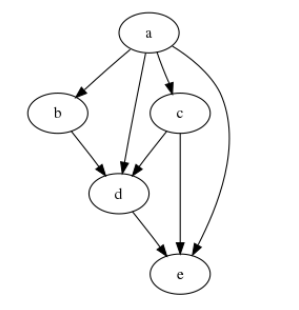
\includegraphics[scale=0.5]{12.png}
\end{figure}

\newpage
Применим алгоритм Кана к графу:
\begin{table}[h!]
    \centering
    \begin{tabular}{|c|c|c|c|c|c|c|c|}
        \hline
        iter & $i$ & $A(a)$ & $A(b)$ & $A(c)$ & $A(d)$ & $A(e)$ & set \\
        \hline
        0 &  & $\varnothing$ & $\{a\}$ & $\{a\}$ & $\{a,b,c\}$ & $\{a,c,d\}$ & $\varnothing$ \\
        \hline
        1 & 1 & $\varnothing$ & $\varnothing$ & $\varnothing$ & $\{b,c\}$ & $\{c,d\}$ & $a$ \\
        \hline
        2 & 2 & $\varnothing$ & $\varnothing$ & $\varnothing$ & $\varnothing$ & $\{d\}$ & $a,b$ \\
        \hline
        3 & 3 & $\varnothing$ & $\varnothing$ & $\varnothing$ & $\varnothing$ & $\varnothing$ & $a,b,c$ \\
        \hline
        4 & 4 & $\varnothing$ & $\varnothing$ & $\varnothing$ & $\varnothing$ & $\varnothing$ & $a,b,c,d$ \\
        \hline
        5 & 5 & $\varnothing$ & $\varnothing$ & $\varnothing$ & $\varnothing$ & $\varnothing$ & $a,b,c,d,e$ \\
        \hline
    \end{tabular}
\end{table}

Результат работы алгоритма: $a, b, c, d, e$.

Пример:
\begin{figure}[h]
    \centering
    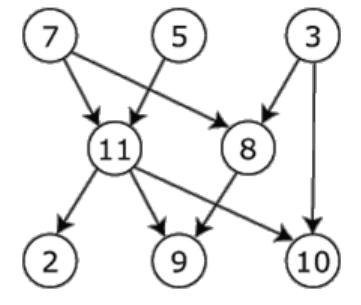
\includegraphics[scale=0.5]{12_2.png}
\end{figure}

Для графа существует несколько согласованных последовательностей его
вершин, которые могут быть получены при помощи топологической
сортировки, например: $7,5,3,11,8,2,9,10; 3,7,5,8,11,10,9,2$.

Видно, что в последовательности могут быть переставлены любые две
стоящие рядом вершины, которые не входят в отношение частичного
порядка (несравнимы)
  \section{Связность в неориентированном графе. Теорема о разложении графа в объединение связных 
подграфов. Компоненты связности графа. Алгоритм нахождения связных компонент графа. 
Найти компоненты связности указанного графа.}

\begin{definition}
    Две вершины в графе называются \textit{связанными}, если существует
    маршрут с началом в первой вершине и концом во второй.
\end{definition}

\begin{definition}
    Граф называется \textit{связным}, если любые две его вершины
    являются связанными.
\end{definition}

\begin{theorem}
    В неориентированном графе отношение связанности на множестве
    вершин является отношением эквивалентности.
    \begin{align*}
        V, \rho = \set{(v_1,v_2),v_1,v_2 \in V, \text{$v_1$ и $v_2$ -- \textit{связанные}}}
    \end{align*}
    \begin{enumerate}[left=0.0em, labelsep=1em, topsep=0.5em, itemsep=0pt, parsep=0.5em]
        \item Рефлексивность -- $\exists$ нуль-маршрут ($\forall v \in V, \; v \rho v$)
        \item Симметричность -- $\exists$ маршрут $ue_1 \dots e_sv$ ($u \rho v$) +
        $\exists$ маршрут $ve_s \dots e_1u$ ($v \rho u$)
        \item Транзитивность -- $\forall u,v,w \in V \; u \rho v \land v \rho w \Rightarrow u \rho w$.
        $\exists$ маршрут $u \dots v$ и $v \dots w \Rightarrow \exists$ маршрут $u \dots w$
    \end{enumerate}
\end{theorem}

\begin{definition}
    Пусть $G(V, E)$ -- граф, то граф $G(V_1,E_1)$ -- подграф графа G, если
    $V_1 \subset V \text{ и } E_1 \subset V$.
\end{definition}

\begin{theorem}
    Любой неориентированный граф распадается в объединение своих
    связных подграфов.
\end{theorem}

\begin{proof}
    Доказано, что в неориентированном графе отношение
    связанности на множестве вершин является отношением эквивалентности.\\
    Известно, что отношение эквивалентности разбивает множество на
    непересекающиеся подмножества - классы эквивалентности, поэтому всё
    множество вершин разбивается на попарно непересекающиеся подмножества
    $V_1,V_2,\dots,V_s, V=V_1 \cup V_2 \cup \dots \cup V_s$.\\
    В каждом таком подмножестве $V_i$ вершины являются связанными. Вершины
    из разных подмножеств не являются связанными. Это, в частности, означает,
    что в графе нет ребер, инцидентных вершинам из разных компонент
    связности. Это и доказывает справедливость утверждения.
\end{proof}

Связные подграфы также называются \textit{связными компонентами графа}.

\textbf{Задача 1.} Доказать, что любой конечный граф имеет чётное количество число
вершин нечётной степени.\\
\textbf{Задача 2.} Доказать, что если в графе только две вершины имеют нечётную
степень, то они связанные.
\begin{proof}
    Докажем, что две вершины, которые имеют нечетную степень, принадлежат
    одной компоненте связности. Предположим противное. Пусть эти вершины
    принадлежат разным компонентам связности. Тогда в подграфах, содержащих
    эти вершины, содержится только одна вершина нечётной степени, что
    противоречит задаче 1.\\
    Поэтому эти вершины принадлежат одной компоненте связности, тогда они
    являются связанными.
\end{proof}

Для нахождения количество связных компонент графа существует алгоритм:
Применяем алгоритм обхода графа в ширину.
\begin{enumerate}[left=0.0em, labelsep=1em, topsep=0.5em, itemsep=0pt, parsep=0.5em]
    \item Всем вершинам графа приписываем значение 0: color(v):=0
    \item k:=0 (количество компонент связности)
    \item Рассматриваем вершины графа.
    Если есть вершина, у которых color(v)=0, то k:=k+1, присваиваем этой
    вершине color(v):=k, заносим вершину в очередь.
    \item Посещается первая вершина из очереди. Всем смежным с ней
    вершинам, у которых color(v)=0, присваиваем color(v):=k и заносим
    в очередь. После этого первая вершина в очереди удаляется из очереди.
    \item Переходим к шагу 4 до тех пор, пока очередь не пуста.
    \item Переходим к шагу 3 до тех пор, пока есть вершины, у которых
    color(v)=0.
    \item Если вершин, у которых color(v)=0, нет, то выводим значение k – число
    компонент связности и stop.
\end{enumerate}

Результатом работы алгоритма является число k -- количество компонент
связности; каждой вершине графа присвоен номер компоненты связности

Иначе говоря: количество запусков алгоритмов в ширину для обхода всего графа
= количеству компонент связности.
  \section{Реберная и вершинная двусвязность графа. Блоки графа, граф блоков – точек сочленения. Найти 
компоненты реберной и вершинной двусвязности, граф блоков – точек сочленения графа.}

Часто при решении прикладных задач теории графов важно, чтобы граф был
“как можно более связным”, то есть при удалении какого-то числа ребер или
вершин он также бы оставался связным. Поэтому кроме понятий связности
существуют также понятия двусвязности, k-связности.

\begin{definition}
    Две вершины в графе называются реберно двусвязными, если
    существует два маршрута с началом в первой вершине и концом во второй, в
    которых нет общих ребер (общие вершины могут быть).
\end{definition}

\begin{definition}
    Граф называется реберно двусвязным, если любые две
    вершины являются реберно двусвязными.
\end{definition}

\begin{theorem}
    В неориентированном графе отношение реберной двусвязности на
    множестве вершин является отношением эквивалентности.
\end{theorem}

\begin{definition}
    Компонентами реберной двусвязности называют его
    подграфы, множества вершин которых -- классы эквивалентности реберной
    двусвязности, а множества ребер -- множества ребер, соединяющих вершины
    соответствующих классов эквивалентности.
\end{definition}

У графа две компоненты связности: $V_1 = \set{1,2,3,4}$ и $V_2 = \set{5,6,7}$:
\begin{figure}[h]
    \centering
    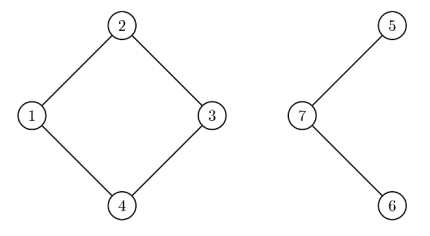
\includegraphics[scale=0.4]{14.png}
\end{figure}

Все вершины первой компоненты реберно двусвязны, поэтому эта компонента
связности является и компонентой реберной двусвязности.

Во второй компоненте никакие две вершины не являются реберно
двусвязными, поэтому каждая из них является отдельной компонентой
реберной двусвязности.

Объединение компонент реберной двусвязности не совпадает с
графом в случае, когда в графе есть мосты.

\begin{theorem}
    Компоненты реберной двусвязности графа $G(V,E)$ -- это
    компоненты связности в графе $G(V,{E}')$, где ${E}'$ получено из $E$ удалением всех
    мостов.
\end{theorem}

То есть для того, чтобы найти компоненты реберной двусвязности в графе
нужно найти все мосты, удалить их из множества ребер графа и в полученном
графе найти все компоненты связности.
  \section{Шарниры и мосты в графе. Алгоритм нахождения мостов в графе. Применить его для графа.}

\begin{definition}
    Вершина в графе называется \textit{разделяющей вершиной} (или
    \textit{точкой сочленения}, или \textit{шарниром}), если её удаление вместе с рёбрами,
    инцидентными ей, приводит к увеличению числа компонент связности.
\end{definition}

\begin{figure}[h]
    \centering
    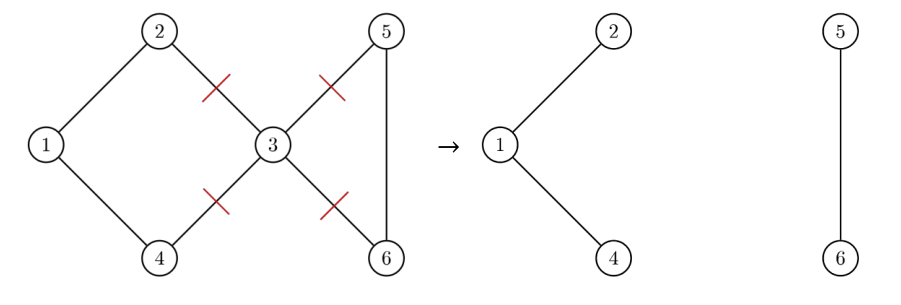
\includegraphics[scale=0.3]{15.png}
\end{figure}

В данном графе вершина 3 является \textit{шарниром}.

\begin{definition}
    \textit{Мостом} в графе называется ребро, удаление которого
    приводит к увеличению числа компонент связности.
\end{definition}

\begin{figure}[h]
    \centering
    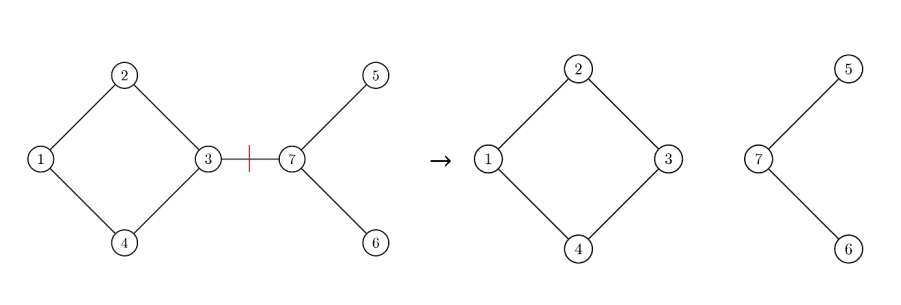
\includegraphics[scale=0.35]{15_2.png}
\end{figure}

Ребро $(3,7)$ является \textit{мостом}.

\newpage
\textbf{Алгоритм нахождения мостов графа:}
\begin{enumerate}[left=0.0em, labelsep=1em, topsep=0.0em, itemsep=0pt, parsep=0.5em]
    \item Проводим поиск в графе в глубину. При появлении новой вершины
    записываем ее в последовательность $L$. При прохождении ребра $(u,v)$ делаем
    ребро ориентированным, а именно, запрещаем прохождение при втором
    поиске в глубину по этому ребру в направлении от вершины $u$ к вершине $v$.
    \item Проводим второй поиск в глубину с учетом ориентированности ребер.
    (если по ребру не проходили, то можно по нему идти в любую сторону).
    Вершины, из которых начинаем обход, берем в порядке из
    последовательности $L$, полученной в шаге 1. Вершинам из одной компоненты
    приписываем один цвет.
    \item Ищем ребра графа, вершины которого раскрашены в разный цвет. Это
    и будут мосты.
\end{enumerate}

Пример алгоритма на графе:
\begin{figure}[h]
    \centering
    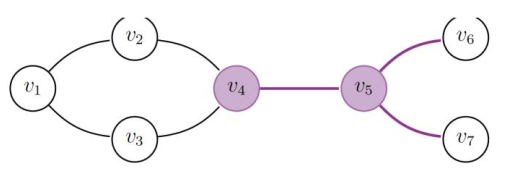
\includegraphics[scale=0.35]{15_3.png}
\end{figure}
\begin{figure}[h]
    \centering
    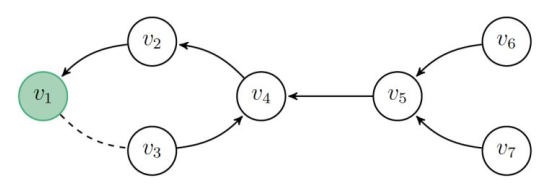
\includegraphics[scale=0.35]{15_4.png}
\end{figure}
\begin{figure}[h]
    \centering
    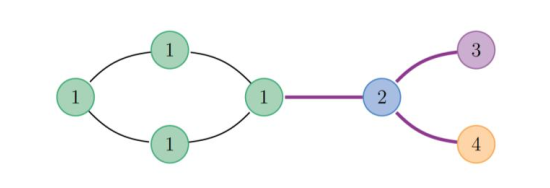
\includegraphics[scale=0.35]{15_5.png}
\end{figure}

Находим ребра, вершины которых раскрашены в разный цвет -- это и будут
мосты: $(4,5), (5,6), (5,7)$.
  \section{Связность в орграфе: различные виды связности, примеры. Компоненты сильной связности. 
Алгоритм Косарайю нахождения компонент сильной связности. Граф конденсации Применить 
алгоритм к орграфу, найти граф конденсации.}
  \section{Теорема о числе маршрутов длины k из одной вершины в другую. Формулировка, 
доказательство. Применить теорему к графу.}

Пусть у графа $G(V,E)$, $|V|=n$, $A$ -- матрица смежности.
Рассмотрим матрицы $A^2,\dots,A^n$, обозначим символом $a_{ij}^{(k)}$ --
элементы матрицы $A^k$.

\begin{theorem}
    Количество маршрутов из $v_i$ в $v_j$ длины $k$ равно числу $a_{ij}^{(k)}$.
\end{theorem}

\begin{proof}
    С помощью методы математической индукции:
    \begin{enumerate}[left=0.0em, labelsep=1em, topsep=0.0em, itemsep=0pt, parsep=0.5em]
        \item $k=1, A=A^1$ \\
        $a_{ij}^{(1)} = s$, где $s$ -- количество ребер, соединяющих вершины $v_i$, $v_j$.
        Поэтому количество маршрутов из $v_i$ в $v_j$ длины 1 равно $s$.

        \item Пусть утвеждение верно для $A^k$ и число маршрутов длины $k$
        равно из $v_i$ в $v_j$ равно $a_{ij}^{(k)}$. Докажем справедливость
        для числа маршрутов длины $k+1$.
        \begin{align*}
            A^{k+1} = A^k \cdot A = 
            \begin{pmatrix}
                a_{11}^{(k)} & \dots & a_{1n}^{(k)}\\
                \hdotsfor[2]{3}\\
                a_{n1}^{(k)} & \dots & a_{nn}^{(k)}
            \end{pmatrix}
            \begin{pmatrix}
                a_{11} & \dots & a_{1n}\\
                \hdotsfor[2]{3}\\
                a_{n1} & \dots & a_{nn}
            \end{pmatrix}
        \end{align*}
        \begin{align*}
            a_{ij}^{(k+1)} = \sum_{t=1}^{n} a_{it}^{(k)}a_{tj}=
            a_{i1}^{(k)}a_{1j} + a_{i2}^{(k)}a_{2j} + \dots + a_{in}^{(k)}a_{nj}
        \end{align*}
        $a_{i1}^{(k)}$ -- количество маршрутов длины $k$ из $v_i$ в $v_1$, $a_{1j}$
        -- количество маршрутов из $v_1$ в $v_j$ длины 1 $\Rightarrow a_{i1}^{(k)}a_{1j}$
        -- количество маршрутов длины $k+1$ из $v_i$ в $v_j$, где последнее ребро $(v_1,v_j)$.
        
        Поскольку последнее ребро может быть либо $(v_1, v_j)$, либо $(v_2, v_j)$,
        либо $(v_n, v_j)$, то по правилу суммы в комбинаторике, получаем
        справедливость утверждения для $k + 1$.

        \item По методу математической индукции заключаем, что теорема верна
        для любого $n \in \mathbb{N}$.
    \end{enumerate}
\end{proof}

\newpage
В любом графе с $n$ вершинами расстояние от любой вершины до любой
другой не более $n-1$. Простой цикл в таком графе имеет длину не больше $n$.
Поэтому справедливы утверждения.

В графе (орграфе) $G$ с $n$ вершинами существует незамкнутый
маршрут из вершины $v_i$ в вершину $v_j$ $(v_i \neq v_j)$ тогда и только тогда, когда
элемент $b_{ij}$ матрицы $A + A^2 + \dots + A^{n-1}$ не равен 0.

В графе (орграфе) $G$ с $n$ вершинами тогда и только тогда
существует цикл, проходящий через вершину $v_i$, когда элемент $b_{ij}$ матрицы
$A + A^2 + \dots + A^n$ не равен нулю.

Пример теоремы к графу:
\begin{figure}[h]
    \centering
    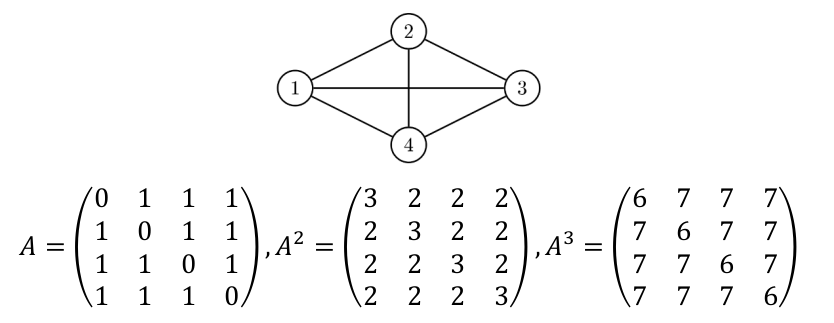
\includegraphics[scale=0.35]{17.png}
\end{figure}

Так как $a_{11}^{(2)}=3$, то существует ровно три маршрута из вершины
1 в 1 длиной 2.
  \section{Матрицы связности и достижимости в графе. Найти матрицу достижимости для указанного 
орграфа, с ее помощью выделить компоненты сильной связности графа.}

Пусть $A$ -- матрица смежности $G$, $|V|=n$. Найдем $B=E+A+A^2+ \dots +A^n$.

Определим матрицу $D$ размерности $n \times n$, $d_{ij}=sign(b_{ij})$.

Эта матрица показывает, есть ли путь из вершины $v_i$ в вершину $v_j$ (в этом
случае $d_{ij}=1$).

\begin{definition}
    В случае если граф $G$ -- неориентированный, матрица $D$
    называется матрицей связности. В случае, если граф $G$ -- ориентированный,
    матрица $D$ называется матрицей достижимости.
\end{definition}

Если $G$ -- неориентированный граф, $v_i \in V$, то в одну компоненту связности с
вершиной $v_i$ входят такие вершины $v_j$, для которых $d_{ij} = 1$.

Можно также ввести матрицу, по которой можно найти компоненты сильной
связности ориентированного графа.

Пусть $D$ -- матрица достижимости орграфа $G, L=D^T$,
\begin{align*}
    l_{ij}&=\begin{cases}
        1,& \text{если есть маршрут из $v_j$ в $v_i$},\\
        0,& \text{если нет}.
        \end{cases} \\
    F &= D \times L, f_{ij}=d_{ij} * l_{ij}.
\end{align*}
Если $f_{ij}$ = 1 , то вершины $v_i$ и $v_j$ принадлежат одной компоненте сильной
связности.

Пример. Рассмотрим ориентированный граф $G(V,E)$
\begin{figure}[h]
    \centering
    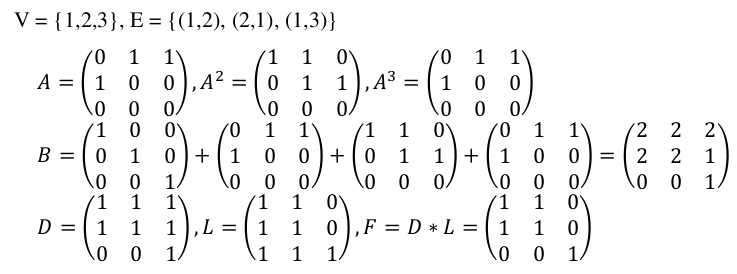
\includegraphics[scale=0.30]{18.png}
\end{figure}

Поэтому у графа 2 компоненты сильной связности $\set{1,2}$ и $\set{3}$.
Это один из способов нахождения компонент сильной связности. Временная
сложность $O(n^4)$.
  \section{Транзитивное замыкание графа. Алгоритм Уоршелла. Применить алгоритм к заданному 
бинарному отношению.}

\begin{definition}
    Транзитивным замыканием бинарного отношения $R$ на
    множестве $M$ называется наименьшее по числу элементов транзитивное
    отношение на множестве $M$, включающее $R$.
\end{definition}

Если изобразить граф бинарного отношения, то транзитивность отношения
означает, что если есть ребра $(u, v), (v, w)$, то есть и ребро $(u, w)$.

На этом может быть основан алгоритм нахождения транзитивного замыкания
бинарного отношения. Для графа можно найти матрицу $T = A + A^2 + \dots + A^n$,
здесь элементы матриц складываем дизьюнктивно:
\begin{align*}
    0+0=0 \vee 0=0; \; 0+1=0 \vee 1=1; \; 1+0=1 \vee 0=1; 1+1=1 \vee 1=1. 
\end{align*}

Если элемент этой матрицы $t_{ij}=1$, то это означает, что существует маршрут от
вершины $v_i$ до $v_j$. Отсюда следует, что для транзитивности отношения эти
вершины в графе должны соединяться ребром.

Поэтому соответствующее этой матрице бинарное отношение и является его
транзитивным замыканием.

Минус этого метода в его временной сложности: временная сложность
нахождения произведения матриц размерности n равна $O(n^3)$, матрицу
смежности нужно умножать на себя n раз, поэтому временная сложность этого
алгоритма $O(n^4)$.

Есть алгоритмы, сложность которых меньше. Опишем один из таких
алгоритмов.

\newpage
\textbf{Алгоритм нахождения транзитивного замыкания Уоршелла}.
\begin{verbatim}
T := А (матрица отношения)
for k = 1 to n do
(Внешний цикл идет по промежуточным вершинам.)
    for i =1 to n do
    (Циклы по i и j перебирают всевозможные пары.)
        for j =1 to n do
            T(i; j) := max {T(i; j), T(i; k) * T(k; j)}
            (Благодаря операции max сохраняются те связи,
            которые были}
        end for
    end for
end for
\end{verbatim}

Трудоемкость такого алгоритма будет $O(n^3)$. Цикл по k нельзя
менять с другими циклами.

\begin{figure}[h]
    \centering
    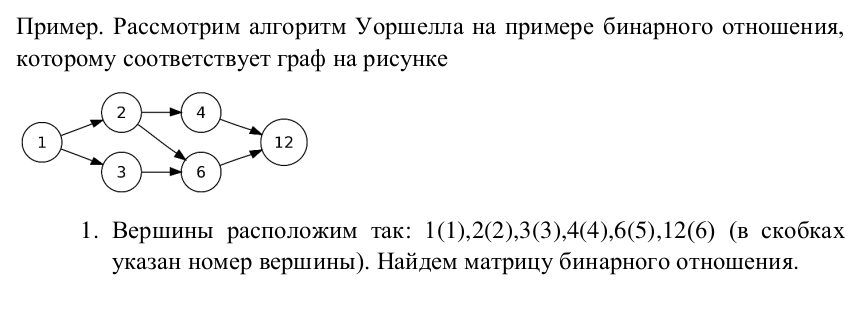
\includegraphics[scale=0.4]{19.png}
\end{figure}
\begin{figure}[h]
    \centering
    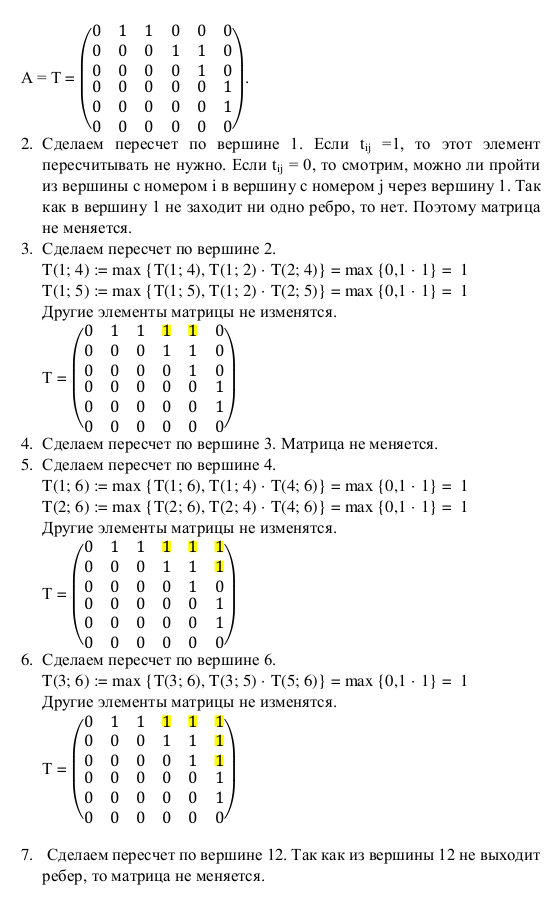
\includegraphics[scale=0.5]{19_2.png}
\end{figure}

В итоге видим, что нужно добавить 5 ребер: (1,4), (1,6), (1,12), (2,12),
(3,12).
  \section{Эйлеровы циклы и цепи в графе. Теорема об эйлеровом цикле. Выяснить, существует ли в графе 
Эйлеров цикл и цепь.}

Задача о Кёнигсбергских мостах послужила началом математической теории
графов.

Изобразим расположение мостов. Задача: выйти из любой точки, пройти по
всем мостам по одному разу и вернуться обратно.

\begin{figure}[h]
    \centering
    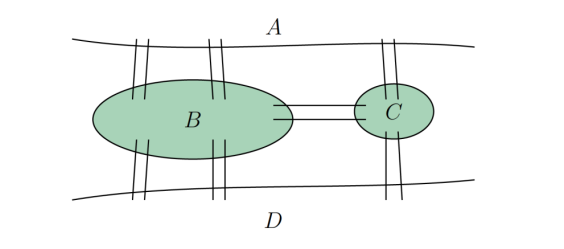
\includegraphics[scale=0.4]{20_1.png}
\end{figure}

Изобразим граф, в котором вершинами является суша, а рёбрами -- мосты.

\begin{figure}[h]
    \centering
    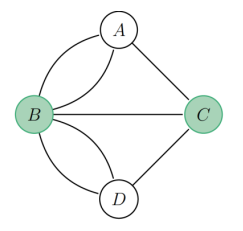
\includegraphics[scale=0.4]{20_2.png}
\end{figure}

\begin{definition}
    Если в графе есть цикл, проходящий по всем рёбрам графа, то
    такой цикл называется \textit{эйлеровым циклом}, а граф называется \textit{эйлеровым
    графом}.
\end{definition}

\begin{theorem}
    Конечный граф без изолированных вершин является эйлеровым
    графом если он является связным и степени всех его вершин четные числа.
    \begin{figure}[h]
        \centering
        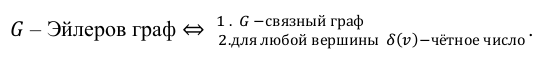
\includegraphics[scale=0.5]{20_3.png}
    \end{figure}
\end{theorem}

\begin{proof}
    $\Rightarrow$ $G$ -- эйлеров граф. По определению, в графе есть эйлеров граф.
    Значит граф связный.

    Каждый раз, проходя через вершину, цикл заходит в эту вершину по одному
    ребру, а выходит по другому ребру. То есть при прохождении через вершину
    задействуется два различных ребра. Так как в эйлеров цикл входят все рёбра
    графа, то степень каждой вершины -- четное число.

    $\Leftarrow$ Пусть граф является связным и степени всех его вершин четные числа.
    Построим в графе $G$ эйлеров цикл. Начнём цикл в произвольной вершине $a$.
    Из вершины $a$ будем строить цикл, проходя всё время по разным рёбрам. Так
    как степень каждой вершины -- чётное число, то цикл может завершиться
    только в вершине $a$.

    Обозначим полученный цикл за P. Если в $P$ входят все рёбра графа $G$, то получили
    эйлеров цикл. Пусть в $P$ входят не все рёбра графа $G$, тогда удалим из графа $G$ все рёбра,
    принадлежащие циклу $P$. Полученный граф обозначим графом $G_1$. Так как в
    графе $G$ степени всех вершин чётные, при прохождении по циклу $P$
    задействуется чётное число рёбер, инцидентных каждой вершине, то в графе $G_1$
    степень каждой вершины также чётна.
    Так как $G$ -- связный граф, то среди вершин цикла $P$ найдётся вершина $b$,
    инцидентная какому то рёбру графа $G_1$.

    Из вершины $b$ в графе $G_1$ снова строим цикл. Получим цикл, который
    завершится в точке $b$. Назовём его ${P}'$. Рассмотрим цикл, полученный
    объединением маршрутов $P(a,b), {P}', P(b,a)$. Получили цикл, содержащий
    больше рёбер, чем в первоначальном. Этот цикл возможно будет эйлеровым.
    Если нет, то процесс продолжим.
    Так как граф конечный, то этот процесс завершится на некотором шаге.
    
    В итоге получим эйлеров цикл.
\end{proof}
  \section{Алгоритм Флери нахождения эйлерова цикла. Применить к указанному графу.}

Рассмотрим один из алгоритмов нахождения эйлерова цикла
-- \textit{алгоритм Флёри}. Он отличается от приведенного алгоритма в
доказательстве теоремы Эйлера тем, что каждый раз при добавлении нового
ребра в марщрут нужно проверять, не является ли это ребро мостом.

В алгоритме нумеруются все ребра графа числами $1,2, \dots , |E|$, так, чтобы
номер, присвоенный данному ребру, указывал, каким по счету это ребро будет
в эйлеровом цикле.

\begin{enumerate}[left=0.0em, labelsep=1em, topsep=0.0em, itemsep=0pt, parsep=0.5em]
    \item Выбираем произвольную вершину $u$, присваиваем произвольному
    ребру $(u,v)$ номер $k=1$. Вычеркиваем это ребро из множества ребер графа и
    переходим в вершину $v$.
    \item Пусть $v$ -- вершина, в которую мы перешли в результате выполнения
    предыдущего шага, $k$ -- номер, присвоенный ребру на этом шаге. Выбираем
    любое ребро, инцидентное вершине v. При этом мост выбираем только в
    случае, когда ребер, инцидентных вершине и не являющихся мостами нет.
    Этому ребру присваиваем номер $k+1$, проходим по нему в следующую
    вершину и вычеркиваем это ребро.
    \item Если в графе есть не вычеркнутые ребра, то переходим к шагу 2, иначе
    stop.
\end{enumerate}

\begin{definition}
    Граф называется \textit{полуэйлеровым}, если в нём существует цель,
    проходящая по всем рёбрам графа.
\end{definition}

\begin{theorem}
    Граф без изолированных вершин называется \textit{полуэйлеровым графом}
    тогда и только тогда, когда выполняется два условия:
    \begin{enumerate}[left=0.0em, labelsep=1em, topsep=0.0em, itemsep=0pt, parsep=0.5em]
        \item Граф $G$ является связным
        \item Только две вершины в графе имеют нечетную степень.
    \end{enumerate}
\end{theorem}

\begin{definition}
    \textit{Полустепенью исхода вершины $v$} орграфа $\delta^-(v)$ называется количество
    рёбер, исходящих из данной вершины.
\end{definition}

\begin{definition}
    \textit{Полустепенью захода вершины $v$}
    орграфа $\delta^+(v)$ называют количество рёбер, заходящих в данную вершину.
\end{definition}

\newpage
Критерий эйлерова и полуэйлерова графа можно дать и для
ориентированного графа без изолированных вершин: для случая
эйлерова графа: полустепени исхода всех вершин должны равняться ее
полустепени захода, граф должен быть сильносвязным; для случая
полуэйлерова графа: полустепени исхода всех вершин, кроме двух
должны равняться полустепени захода, для одной из оставшихся вершин
полустепень исхода на единицу больше полустепени захода, для другой
вершины наоборот.
  \section{Графы де Брюина: определение, свойства, алгоритм построения. Применение для построения 
слова наименьшей длины, которое содержит все указанные подслова.}

\begin{definition}
    Конечное множество символов $A = \set{a_1, a_2,\dots,a_n}$ называют
    алфавитом, символы алфавита -- буквами, последовательность символов
    алфавита -- словами. Число символов в слове называют длиной слова.
\end{definition}

\begin{definition}
    Пусть задан алфавит, состоящий из $n$ букв. Графом де Брюина
    (обозначается $B(n,k)$) для алфавита $A$ называется ориентированный граф
    $G(V,E)$, множеством вершин которого является множество слов длины $k$ в
    алфавите $A$. Ребро (дуга) из вершины $u$ в вершину $v$ проводится, если 
    \begin{align*}
        u = \set{x_1x_2 \dots x_k} , v = \set{y_1y_2 \dots y_k} \\
        x_2 = y_1, x_3=y_2,\dots, x_k=y_k-1.
    \end{align*}
\end{definition}

Это означает, что если вершина $u = \set{x_1x_2 \dots x_k}$,
то вершина \\ $v = \set{x_2x_3 \dots x_ky_k}$,
при этом ребру $(u, v)$ сопоставляется последовательность из $k+1$ символа:
$e = (u, v) = {x_1x_2 \dots x_ky_k}$.

Вершина $u$ называется префиксом, а вершина $v$ -- суффиксом слова $e$.

Справдливы следующие теоремы.

\begin{theorem}
    Граф де Брюина является эйлеровым графом.
\end{theorem}

\begin{theorem}
    Граф де Брюина содержит $n^k$ вершин и $n^{k+1}$ ребер.
\end{theorem}

\textbf{Алгоритм построения графа де Брюина}
\begin{enumerate}[left=0.0em, labelsep=1em, topsep=0.0em, itemsep=0pt, parsep=0.5em]
    \item Генерируем в любом порядке все слова длины $k+1$ в алфавите $A$.
    \item Для каждого слова(ребра) $\set{x_1x_2 \dots x_kx_{k+1}}$ определяем вершины (узлы):
    $u = {x_1x_2 \dots x_k}, v={x_2x_3 \dots x_kx_{k+1}}$.
\end{enumerate}

Пример: Пусть $A=\set{a,b}, k=2$. Получаем следующие ребра и вершины графа:
\begin{table}[h!]
    \centering
    \begin{tabular}{|c|c||c|c|}
    \hline
    \textbf{Слово} & \textbf{Узлы} & \textbf{Слово} & \textbf{Узлы} \\
    \hline
    \{aaa\} & \{aa\} $\to$ \{aa\} & \{baa\} & \{ba\} $\to$ \{aa\} \\
    \{aab\} & \{aa\} $\to$ \{ab\} & \{bab\} & \{ba\} $\to$ \{ab\} \\
    \{aba\} & \{ab\} $\to$ \{ba\} & \{bba\} & \{bb\} $\to$ \{ba\} \\
    \{abb\} & \{ab\} $\to$ \{bb\} & \{bbb\} & \{bb\} $\to$ \{bb\} \\
    \hline
    \end{tabular}
\end{table}

Изобразим полученный граф:
\begin{figure}[h]
    \centering
    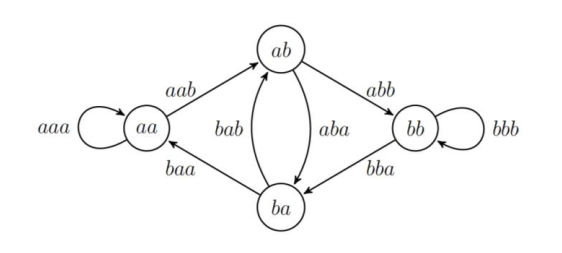
\includegraphics[scale=0.4]{22.png}
\end{figure}

Пример: При помощи графа де Брюина найти слово наименьшей длины,
которое содержит все подслова из множества \\ 
$R=\set{ACT,CTG,TGA,GAC,ACG,CGA}$.

По алгоритму:
\begin{enumerate}[left=0.0em, labelsep=1em, topsep=0.0em, itemsep=0pt, parsep=0.5em]
    \item $V = \set{AC, CT, TG, GA, CG}$ -- вершины графа.
    \item Строим граф.
    \begin{figure}[h]
        \centering
        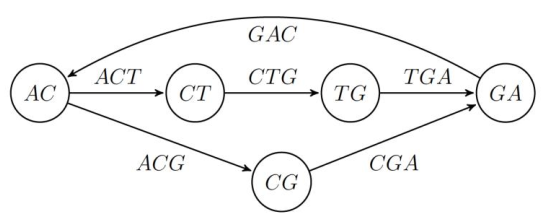
\includegraphics[scale=0.4]{22_2.png}
    \end{figure}
    \item Строим эйлерову цепь: $AC \to CT \to TG \to GA \to AC \to CG \to GA$
    Замечание. Эйлерову цепь начинаем в вершине, из которой выходит на
    одно ребро больше, чем заходит в вершину.
    \item Построенной эйлеровой цепи соответствует слово минимальной длины,
    которое содержит все подслова из $R: ACTGACGA$
    (Cтроим по правилу: $AC+T+G+A+C+G+A$)
\end{enumerate}


  \section{Гамильтоновы циклы и цепи в графе. Теоремы Дирака и Оре. Выяснить, существует ли в 
указанном графе Гамильтонов цикл.}

\begin{definition}
    Граф называется \textit{гамильтоновым}, если существует простой
    цикл, проходящий по всем вершинам графа.
\end{definition}

\begin{definition}
    Граф называется \textit{полугамильтоновым}, если существует простая
    цепь, проходящая через все вершины графа.
\end{definition}

Покажем, что понятия эйлерова и гамильтонова графа не связаны между
собой, то есть у графов могут встретиться всевозможные комбинации этих
понятий.

\begin{figure}[h]
    \centering
    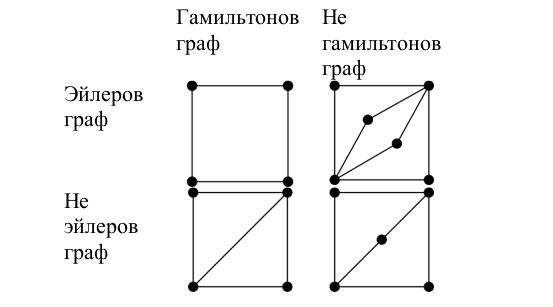
\includegraphics[scale=0.4]{23.png}
\end{figure}

Критерия гамильтонова графа нет. Но есть достаточные условия
гамильтоновости графа. Теоремы Дирака и Оре связывают понятие
гамильтоновости со степенями $\delta(v)$ вершин графа.

\begin{theorem}
    \textbf{Дирака}. Если $n \geq 3$ и $\delta(v) \geq n/2$ для любой вершины $v$
    неориентированного графа $G$, то $G$ -- гамильтонов граф.
\end{theorem}

\begin{theorem}
    \textbf{Оре}. Если $n \geq 3$ и $\delta(u) + \delta(v) \geq n$ для любых двух различных
    несмежных вершин $u, v$ неориентированного графа $G$, то $G$ -- гамильтонов граф.
\end{theorem}
  \section{Деревья. Теорема о связи вершин и ребер в дереве.}

\begin{definition}
    Граф называется \textit{деревом}, если он является связным и не
    содержит циклов.
\end{definition}

\begin{definition}
    Граф, все компоненты связности которого являются деревьями,
    называется \textit{лесом}.
\end{definition}

\begin{theorem}
    Пусть граф $G$ -- дерево, у которого $n$ вершин и $r$ ребер. Тогда
    справедливо равенство $r = n - 1$.
\end{theorem}

\begin{proof}
    Методом математической индукции:
    \begin{enumerate}[left=0.0em, labelsep=1em, topsep=0.0em, itemsep=0pt, parsep=0.5em]
        \item $G$ -- дерево. $n=1$. Так как петель в дереве не может быть, то $r=0$.
        \item Пусть равенство выполняется для дерева с $n = k$ вершинами. То есть у
        такого дерева $r = k - 1$ ребер. Докажем, что равенство будет выполняться
        и для дерева $G$ с $k+1$ вершиной.
        \item В дереве $G$ существует ребро, поэтому есть и висячая вершина. Эта
        вершина не является шарниром, поэтому после ее удаления вместе с
        инцидентным ему ребром граф останется связным. Очевидно также, что
        в полученном после удаления вершины и ребра графе не будет циклов
        (так как их нет в $G$). Поэтому полученный граф является деревом с k
        вершинами. Известно, по предположению индукции, что у него $k - 1$
        ребро. У графа $G$ на одну вершину и на одно ребро больше, поэтому y
        него $k+1$ вершина и $k$ ребер, то есть число ребер на единицу меньше
        числа вершин.
        \item По методу математической индукции заключаем, что утверждение
        справедливо для любого дерева.
    \end{enumerate}
\end{proof}

Задача №1. В любом дереве, в котором есть хотя бы одно ребро, есть висячие
вершины.

Задача №2. Висячая вершина не является шарниром.
  \section{Остовное дерево связного графа. Минимальное остовное дерево. Алгоритмы Прима и Краскала, 
их применение.}

\begin{definition}
    \textit{Остовным (стягивающим) деревом} связного графа называется
    его подграф, содержащий все вершины графа и являющийся деревом.
\end{definition}

\begin{definition}
    Если каждому ребру графа сопоставляется какое-то число
    (называют вес или длина или стоимость ребра), то такой граф называется
    \textit{нагруженным (взвешенным) графом}.
\end{definition}

Обозначение: $l(e)$ -- длина ребра, $w(e)$ -- вес ребра.

Пример нагруженного графа и его остовного дерева
\begin{figure}[h]
    \centering
    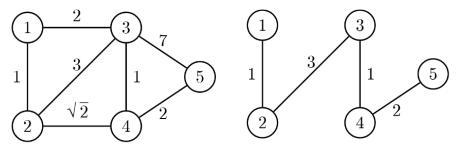
\includegraphics[scale=0.4]{25_1.png}
\end{figure}

Пусть $G$ -- нагруженный граф.

\begin{definition}
    \textit{Минимальным остовным деревом нагруженного графа}
    называется остовное дерево с минимальной суммой длин входящих в него
    ребер.
\end{definition}

Опишем алгоритмы Прима и Краскала, которые позволяют находить
минимальное остовное дерево нагруженного графа.

Алгоритмы Прима и Краскала называются также \textit{жадными алгоритмами}, то
есть алгоритмами, при которых на каждом шаге происходит поиск
оптимального выбора.

\textbf{Алгоритм Прима нахождения минимального остовного дерева.}
Пусть в нагруженном графе $G$ число вершин равно $n$.
\begin{enumerate}[left=0.0em, labelsep=1em, topsep=0.0em, itemsep=0pt, parsep=0.5em]
    \item Берем произвольную вершину графа. Находим в графе $G$ ребро
    минимальной длины, инцидентное этой вершине. Получаем подграф,
    состоящий из 2 вершин и ребра, соединяющего эти вершины. Обозначим этот
    подграф $G_2$, $i:=2$.
    \item Если $i=n$, то останавливаемся. Если нет, то переходим к шагу 3.
    \item Рассмотрим рёбра графа $G$, одна из вершин которых принадлежит
    графу $G_i$, а вторая не принадлежит. Из всех таких рёбер выбираем ребро
    минимальной длины и добавляем его к графу $G_i$. Получаем граф $G_{i+1}$, $i:=i+1$.
    Переходим к шагу 2.
\end{enumerate}

Пример. Найдем минимальное остовное дерево с помощью алгоритма Прима:
\begin{figure}[h]
    \centering
    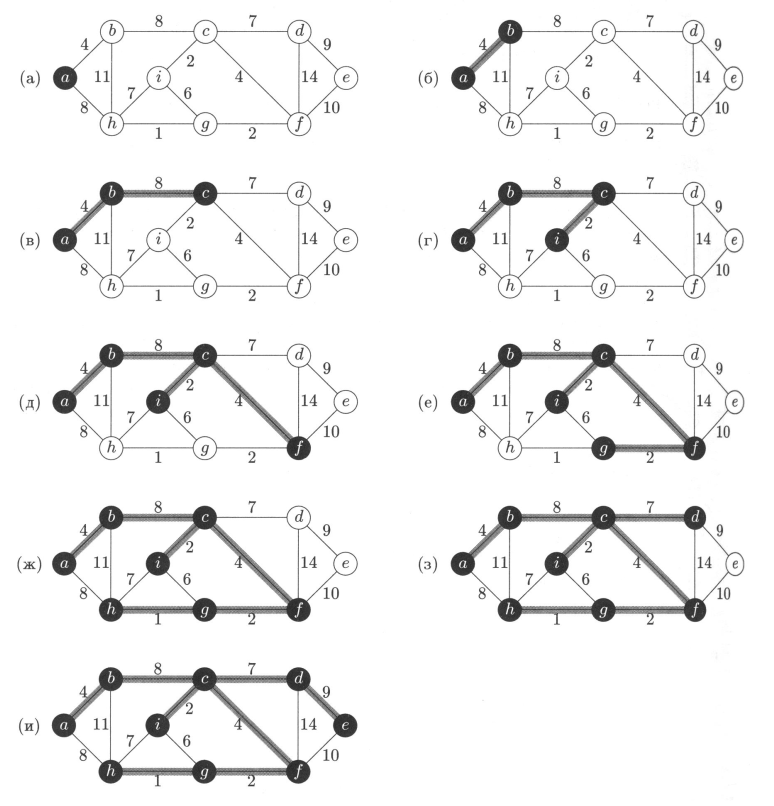
\includegraphics[scale=0.40]{25_2.png}
\end{figure}

Найдем длину(вес) полученного остовного дерева:

$4+8+7+9+2+4+1+2=37$

\newpage
\textbf{Алгоритм Краскала (Крускала) нахождения минимального остовного
дерева.}

Пусть в нагруженном графе $G$ число вершин равно $n$.
\begin{enumerate}[left=0.0em, labelsep=1em, topsep=0.0em, itemsep=0pt, parsep=0.5em]
    \item Упорядочиваем все ребра графа $G$ в порядке неубывания -- от ребер
    минимальной длины к максимальной. Множество ребер остовного дерева
    пусто.
    \item Первое ребро в остовном дереве - первое из упорядоченного списка (то
    есть ребро минимальной длины).
    \item Если в множестве ребер содержится $n-1$ ребер, то останавливаемся.
    Если нет, то переходим к шагу 4.
    \item Добавим в множество ребер остовного дерева такое ребро
    минимальной длины из оставшихся ребер, при добавлении которого не
    появятся циклы. Переходим к шагу 3.
\end{enumerate}

Пример. Найдем минимальное остовное дерево с помощью алгоритма
Краскала:
\begin{figure}[h]
    \centering
    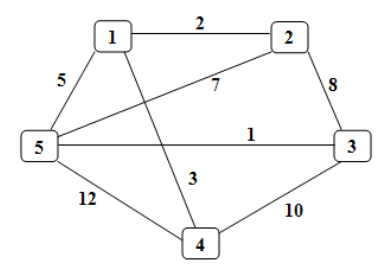
\includegraphics[scale=0.35]{25_3.png}
\end{figure}
\begin{enumerate}[left=0.0em, labelsep=1em, topsep=0.0em, itemsep=0pt, parsep=0.5em]
    \item Упорядочиваем ребра: $(5,3), (1,2), (1,4), (1,5), (5,2), (2,3), (3,4), (5,4)$.
    \item $V$ -- множество вершин, $E$ -- множество ребер остовного дерева. $V=\varnothing,E=\varnothing$.
    \item $E = \set{(5,3)}, V = \set{5,3}$
    \item $E = \set{(1,2), (5,3)}, V = \set{1,2,5,3}$
    \item $E = \set{(1,2), (5,3), (1,4)}, V = \set{1,2,5,3,4}$
    \item $E = \set{(1,2), (5,3), (1,4), (1,5)}, V = \set{1,2,5,3,4}$
    \item $n-1$ ребер, stop.
\end{enumerate}

Найдем длину (вес) полученного остовного дерева: $1+2+3+5=11$.
  \section{Матрица Кирхгофа, ее применение для нахождения числа остовных деревьев. Корневые деревья: 
основные определения. Найти число остовных деревьев с помощью матрицы Кирхгофа.}

Пусть $G$ -- связный неориентированный граф. $|V| = n$.

\begin{definition}
    \textit{Матрицей Кирхгофа} графа $G$ называется квадратная матрица
    размерности $n \times n$, в которой
    \begin{align*}
        b_{ij}&=\begin{cases}
            k,&  \text{где $\delta(v_i)=k, i=j$},\\
            -1,& \text{если $i \neq j$, $v_i$ и $v_j$ смежны}, \\
            0,&  \text{если $v_i$ и $v_j$ не смежны}.
            \end{cases}
    \end{align*}
\end{definition}

\begin{theorem}
    Число остовных деревьев в связном графе $G$, равно алгебраическому
    дополнению любого элемента матрицы Кирхгофа.
\end{theorem}

Пример. Изобразить граф, заданный с помощью матрицы Кирхгофа, найти
число остовных деревьев графа и их изобразить.
\begin{figure}[h]
    \centering
    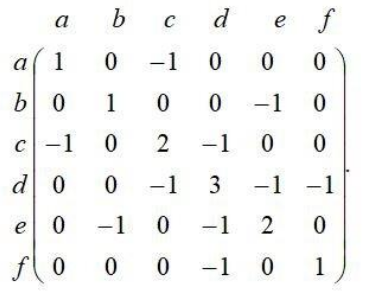
\includegraphics[scale=0.4]{26.png}
\end{figure}

Найдем алгебраическое дополнение элемента матрицы с индексом 44.

$A_{44} = 1$. Это означает, что существует лишь одно остовное дерево этого графа.
Это остовное дерево является самим графом.

\newpage
\textbf{Корневые деревья}
\begin{definition}
    \textit{Корневым деревом} называют дерево с выделенной вершиной --
    корнем.
\end{definition}

\begin{definition}
    Висячую вершину корневого дерева называют \textit{листом}.
    \textit{Высотой корневого дерева} называют расстояние от корня до самого
    удаленного листа. Если в корневом дереве маршрут, соединяющий вершину $u$
    c корнем, проходит через вершину $v$, то говорят, что вершина u -- \textit{потомок
    вершины} $v$, вершина $v$ -- \textit{предок вершины} $u$. Множество всех потомков
    вершины $v$ является деревом с корнем $v$, оно называется \textit{ветвью дерева} в
    вершине $v$. Если предок и потомок соединены ребром, то они называются
    \textit{отцом и сыном}.
\end{definition}

На рисунке пример дерева, в котором выделили вершину $v_4$ и оно стало
корневым деревом. Обычно корень принято изображать сверху (как в
генеалогическом древе). Иногда его изображают внизу.

\begin{figure}[h]
    \centering
    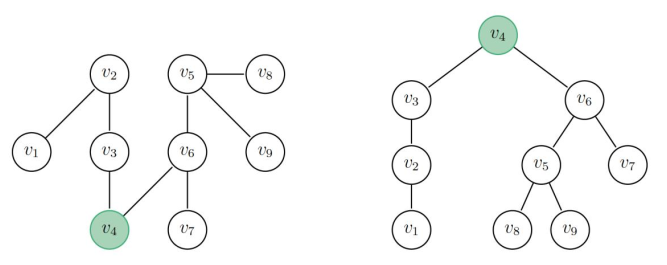
\includegraphics[scale=0.4]{26_2.png}
\end{figure}

У графа на рисунке высота корневого дерева равна трем.

Для вершин $v_1$ и $v_3$, вершина $v_1$ -- \textit{потомок} вершины $v_3$, вершина $v_3$ \textit{предок}
вершины $v_1$, вершина $v_2$ -- \textit{отец} вершины $v_1$.

Множество вершин $\set{v_1, v_2, v_3}$ всех потомков вершины $v_3$ является деревом с
корнем $v_3$, оно является ветвью дерева в вершине $v_3$.

\begin{definition}
    Ориентированным деревом называют ориентированный граф
    без циклов, в котором в каждую вершину, кроме одной, называемой корнем,
    входит ровно одно ребро. В корень ориентированного дерева не входит ни
    одного ребра.
\end{definition}

Иногда ориентированные деревья изображают с вершиной -- корнем
внизу, ребра также могут быть изображены направленными в сторону корня.
  \section{Теорема Кэли о числе помеченных деревьев. Код Прюфера для дерева: алгоритмы кодирования и 
декодирования, его применение.}

\begin{definition}
    Граф называется \textit{помеченным (пронумерованным)}, если каждой
    вершине графа сопоставляется некая метка (если у графа $n$ вершин, то метки
    -- это числа от $1$ до $n$).
\end{definition}

При изоморфизме помеченных графов вводится дополнительное условие:
пары вершин первого и второго графов с одинаковыми метками должны быть
смежны одновременно.

\begin{theorem}
    \textbf{Кэли:} Число различных помеченных деревьев с $n$ вершинами равно
    $n^{n-2}$.
\end{theorem}

Укажем алгоритм, по которому можно для помеченных деревьев с $n$
вершинами $(n \geq 3)$ указать его код, состоящий из $n$ -- 2 чисел (числа могут
повторяться).

Алгоритм нахождения \textbf{кода Прюфера} помеченного дерева:

\begin{enumerate}[left=0.0em, labelsep=1em, topsep=0.0em, itemsep=0pt, parsep=0.5em]
    \item Находим в дереве висячую вершину с минимальным номером.
    Удаляем эту вершину вместе с инцидентным ей ребром из графа. Номер
    смежной ей вершины записываем в код.
    \item Если в графе осталось 1 ребро, то останавливаем алгоритм. Если нет,
    то переходим к шагу 1.
\end{enumerate}

Найдем код Прюфера для следующего дерева:
\begin{figure}[h]
    \centering
    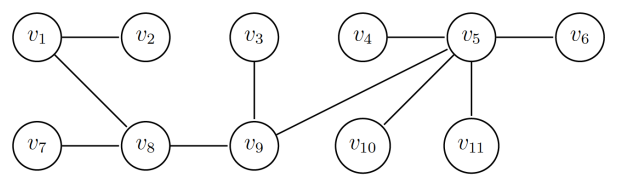
\includegraphics[scale=0.35]{27.png}
\end{figure}

\begin{table}[h!]
    \centering
    \begin{tabular}{|c|c|c||c|c|c||c|c|c|}
    \hline
    $i$ & Вершина & $p_i$ & $i$ & Вершина & $p_i$ & $i$ & Вершина & $p_i$ \\
    \hline
    1 & $v_2$ & 1 & 4 & $v_4$ & 5 & 7 & $v_8$ & 9 \\
    2 & $v_1$ & 8 & 5 & $v_6$ & 5 & 8 & $v_9$ & 5 \\
    3 & $v_3$ & 9 & 6 & $v_7$ & 8 & 9 & $v_{10}$ & 5 \\
    \hline
    \end{tabular}
\end{table}

Получаем следующий код Прюфера: $P=\set{1,8,9,5,5,8,9,5,5}$

В код Прюфера входят только вершины, не являющиеся висячими.
При этом они участвуют в коде $\delta(v)$ -- 1 раз.

\textbf{Алгоритм восстановления дерева:}
\begin{enumerate}[left=0.0em, labelsep=1em, topsep=0.0em, itemsep=0pt, parsep=0.5em]
    \item Записываем код дерева в первой строке. Находим количество вершин
    в дереве (число чисел в коде плюс 2) Во второй строке выписываем вершины,
    которых нет в коде (висячие вершины).
    \item Берём вершину $u$ -- первую вершину в первой строке и вершину $v$ --
    вершину с минимальным номером из второй строки. Записываем ребро $(u, v)$
    и вычёркиваем $u$ и $v$ из соответствующих строк. Если вершины $u$ больше нет
    в первой строке, то записываем её во вторую строку.
    \item Если вершин в первой строке не осталось, то из оставшихся двух
    вершин нижней строки составляем ребро и останавливаем алгоритм, иначе
    переходим к шагу 2.
\end{enumerate}

Пример. Восстановим дерево по коду Прюфера из примера выше.
\begin{multicols}{2}
    \begin{enumerate}[left=0.0em, labelsep=1em, topsep=0.0em, itemsep=0pt, parsep=0.5em]
        \item Записываем код в первой строке, висячие вершины во второй:\\
        \textbf{1},8,9,5,5,8,9,5,5 (n=11)\\
        \textbf{2},3,4,6,7,10,11
        \item Записываем ребро (1,2)\\
        \textbf{8},9,5,5,8,9,5,5\\
        3,4,6,7,10,11,\textbf{1}
        \item Записываем ребро (8,1)\\
        \textbf{9},5,5,8,9,5,5\\
        \textbf{3},4,6,7,10,11
        \item Записываем ребро (9,3)\\
        \textbf{5},5,8,9,5,5\\
        \textbf{4},6,7,10,11
        \item Записываем ребро (5,4)\\
        \textbf{5},8,9,5,5\\
        \textbf{6},7,10,11
        \item Записываем ребро (5,6)\\
        \textbf{8},9,5,5\\
        \textbf{7},10,11
        \item Записываем ребро (8,7)\\
        \textbf{9},5,5\\
        10,11,\textbf{8}
        \item Записываем ребро (9,8)\\
        \textbf{5},5\\
        10,11,\textbf{9}
        \item Записываем ребро (5,9)\\
        \textbf{5}\\
        \textbf{10},11
        \item Записываем ребро (5,10)\\
        11,5
        \item Записываем ребро (5,11)
    \end{enumerate}
\end{multicols}

Получили граф, соответствующий графу, код которого получали в
предыдущем примере.
  \section{Цикломатическое число графа, теорема о связи цикломатического числа с количеством вершин, 
ребер и компонент связности.}

\begin{definition}
    \textit{Цикломатическим числом графа} называется минимальное
    число рёбер, которое нужно удалить, чтобы в графе не было циклов.
\end{definition}

Если граф $G$ -- связный, то нужно удалить рёбра так, чтобы получилось
остовное дерево графа.

\begin{theorem}
    Цикломатическое число графа, у которого $n$ вершин, $r$ рёбер и $k$
    компонент связности, равно $r - n + k$.
\end{theorem}

\begin{proof}
    Рассмотрим сначала случай, когда граф $G$ -- связный, у него
    $n$ вершин и $r$ рёбер, одна компонента связности. Для того, чтобы у подграфа
    этого графа не было циклов, нужно удалить рёбра так, чтобы получилось
    остовное дерево графа.

    Пусть $s$ -- количество рёбер, которые нужно удалить, чтобы получить остовное
    дерево. Из общего числа ребер $r$ вычитаем число ребер в остовном дереве.
    Известно, что их $n - 1$.
    \begin{align*}
        s = r - (n - 1) = r - n + 1 \text{-- цикломатическое число связного графа}.
    \end{align*}
    Обозначим цикломатическое число графа $\mu(G)$.

    Пусть теперь $G(V, E)$ -- граф, у которого $n$ вершин, $r$ рёбер и $k$ компонент
    связности. Тогда нам нужно получить остовной лес. Для этого в каждой
    компоненте связности ищем его остовное дерево. Обозначим $n_i$ и $r_i$ --
    количество вершин и ребер в компоненте связности с номером $i$. Тогда
    цикломатическое число равно:
    \begin{multline*}
        \mu(G) = (r_1 - n_1 +1) + (r_2 - n_2 + 1) + \dots + (r_k - n_k + 1) =\\
        = (r_1 + r_2 + \dots + r_k) - (n_1 + n_2 + \dots + n_k) + k = r - n + k.
    \end{multline*}
\end{proof}
  \section{Главные циклы графа, Теорема о разложении цикла в сумму главных циклов. Применение для 
указанного графа.}

\begin{definition}
    Пусть $G (V, E)$ -- связный граф с $n$ вершинами и $r$ ребрами,
    $T (V, E_1)$ -- остовное дерево графа $G$. Ребра $e \in E_1$ называются \textit{ветвями}, ребра
    $y \in E \setminus E_1$ называются \textit{хордами} графа.
\end{definition}

Если к остовному дереву добавить хорду $y = (u,v)$, то $y$ и $T$ образуют граф с
циклом, который определяется единственным образом цепью, соединяющей
вершины $u$ и $v$. Этот цикл называют \textit{главным циклом, определяемым хордой y}.

Множество всех главных циклов называют \textit{фундаментальной системой
циклов}.

Ветвей в графе $n-1$, тогда хорд $r - (n - 1) = r - n + 1 = \mu(G)$ --
цикломатическое число графа.

\begin{definition}
    Введем операцию сложения по модулю 2 над множествами
    ребер графа $M_1$ и $M_2$:
    \begin{align*}
        M_1 \oplus M_2 = \set{e \in E | (e \in M_1 \text{ и } e \notin M_2) \text{ или } (e \notin M_1 \text{ и } e \in M_2)}.
    \end{align*}
\end{definition}
Эту операцию можно задать и для произвольного конечного числа
подмножеств ребер графа: ребро будет принадлежать сумме подмножеств
ребер, если оно принадлежит нечетному числу подмножеств.

\begin{theorem}
    Любой цикл Z графа является суммой его некоторых главных
    циклов:
    \begin{align*}
        Z = C_{i_1} \oplus \cdots \oplus C_{i_k}.
    \end{align*}
\end{theorem}

Пример. Рассмотрим граф на рисунке. Ребра остовного дерева обозначены
зеленым цветом. Построим главные циклы графа.
\begin{figure}[h]
    \centering
    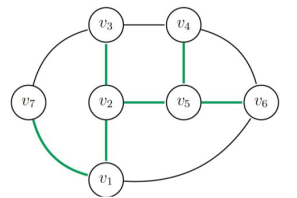
\includegraphics[scale=0.4]{29.png}
\end{figure}

Рассматриваем все хорды графа. Добавляем их по очереди в остовное дерево,
смотрим, какой цикл получился, записываем его.
\begin{align*}
    C_1 &- (v_3,v_4): v_3 \rightarrow v_4 \rightarrow v_5 \rightarrow v_2 \rightarrow v_3\\
    C_2 &- (v_4,v_6): v_4 \rightarrow v_6 \rightarrow v_5 \rightarrow v_4\\
    C_3 &- (v_1,v_6): v_1 \rightarrow v_6 \rightarrow v_5 \rightarrow v_2 \rightarrow v_1\\
    C_4 &- (v_3,v_7): v_3 \rightarrow v_2 \rightarrow v_1 \rightarrow v_7 \rightarrow v_3
\end{align*}

Получили четыре главных цикла. $C_1, C_2, C_3, C_4$ - фундаментальная система
циклов. Через нее можно выразить любой цикл.
\begin{align*}
    \text{Рассмотрим цикл } Z &= \set{v_1 \rightarrow v_2 \rightarrow v_3 \rightarrow v_4 \rightarrow v_6 \rightarrow v_1}.
    \text{ Тогда}\\
    Z &= C_1 \oplus C_2 \oplus C_3.
\end{align*}
Для того, чтобы найти разложение цикла $Z$ в сумму главных
циклов, нужно взять те циклы, которым принадлежат хорды, входящие в цикл
$Z$.
  \section{Укладка графа. Планарные и плоские графы. Теорема Эйлера о связи числа вершин, ребер и 
граней в плоском графе.}


  \section{Следствие из теоремы Эйлера о связи числа вершин, ребер и граней в плоском графе.  Доказать, 
что для графов - триангуляций выполняется верхняя оценка следствия.}

Теорема Эйлера справедлива для любых псевдографов, следствие из нее
справедливо только для простых графов.

\textbf{Следствие:}
Если связный простой плоский граф имеет $n$ вершин, где $n \geq 3$ и
$r$ ребер то справедливо неравенство: $3n - r \geq 6$.

\begin{proof}
    Обозначим через qk число граней, ограниченных k ребрами.
    Так как в графе нет петель и кратных ребер, то $q_1 = q_2 = 0$. Поэтому число всех
    граней равно: $q = q_3 + q_4 + \dots$.

    Покажем, что справедливо равенство $2r = 3q_3 + 4q_4 + \dots$.

    В нем справа найдено количество всех ребер, ограничивающих каждую
    грань. Так, q3 – количество граней, ограниченных 3 ребрами, поэтому $3q_3$ --
    количество всех ребер, ограничивающих эти грани. Каждое ребро в этой
    сумме учитывается дважды, так как каждое ребро принадлежит двум граням
    (или два раза одной грани), поэтому слева стоит множитель 2.
    Получаем: $2r = 3q_3 + 4q_4 + \dots \geq 3(q_3 + q_4 + \dots) = 3q$.
    Поэтому $2r \geq 3q$, поэтому $q \geq \frac{2}{3}r$.

    По теореме Эйлера $n-r+q=2$. Тогда $q = 2 - n + r \geq \frac{2}{3}r$.

    $6 - 3n + 3r - 2r \geq 0$, поэтому получаем: $3n - r \geq 6$.
\end{proof}

В следствии доказывается, что если связный плоский граф имеет
$n$ вершин, где $n \geq 3$ и $r$ рёбер, то справедливо неравенство: $3n - r \geq 6$.

В связи с этим возникает вопрос: существуют ли графы с верхней оценкой,
то есть для любого ли n существует планарный граф, для которого верно
$3n - r = 6$. Оказывается, существуют.

\begin{definition}
    Это связные планарные графы, в которых любая грань (включая внешнюю)
    ограничена циклом длины 3. Такие графы называются \textit{триангуляциями}.
\end{definition}

\newpage
Докажем методом математической индукции по числу вершин $n$, где $n \geq 3$,
что для таких графов равенство $3n - r = 6$ выполняется.

\begin{enumerate}[left=0.0em, labelsep=1em, topsep=0.0em, itemsep=0pt, parsep=0.5em]
    \item Если $n=3$, то таким графом является полный граф $К_3$. Для него $9-3 =6$.
    \item Пусть для n у такого графа равенство выполняется: $3n - r =6$. Докажем,
    что для такого графа с $n+1$ вершиной равенство также будет
    выполняться.
    К имеющемуся графу с $n$ вершинами добавляем одну вершину. Она
    попадет в один из треугольников. Соединяем ее с тремя вершинами
    треугольника, внутрь которого она попала, при этом планарность не
    нарушается. Таким образом, добавляется 3 ребра, то есть у графа $(n+1)$
    вершина и $(r+3)$ ребра.
    \begin{align*}
        3(n+1) - (r+3) = 3n + 3 - r - 3 = 3n - r =6.
    \end{align*}
    \item По методу математической индукции заключаем, что равенство
    справедливо для любого $n$.
\end{enumerate}

\textbf{Пример:} Для графа на рисунке удостовериться, что справедлива формула
Эйлера, равенство $2r = 3q_3 + 4q_4 + \dots$ и неравенство $3n - r \geq 6$.
\begin{figure}[h]
    \centering
    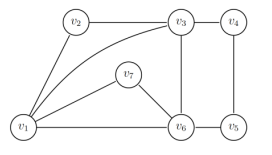
\includegraphics[scale=0.5]{31.png}
\end{figure}

$n=7, r = 10, q=5. 7-10+5 =2$ (верно)\\
$q_3 =2, q_4 = 2, q_6 = 1$ (внешняя грань)\\
$20 = 3 \cdot 2+ 4 \cdot 2 + 6 \cdot 1 = 6+8+6$ (верно)\\
$3 \cdot 7 - 10 \geq 6$ (верно)
  \section{Доказательство непланарности графов $K_5$ и $K_{3,3}$. Критерий планарности графов. Выяснить, 
является ли граф планарным.}

С помощью следствия из теоремы Эйлера можно доказать непланарность
некоторых графов.

Рассмотрим полный граф $K_5$. У него $n=5, r=10$.
\begin{figure}[h]
    \centering
    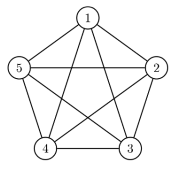
\includegraphics[scale=0.4]{32_1.png}
\end{figure}

$3 \cdot 5 - 10 = 5 < 6$, поэтому этот граф не является планарным.

Рассмотрим полный двудольный граф $K_{3,3}$.
\begin{figure}[h]
    \centering
    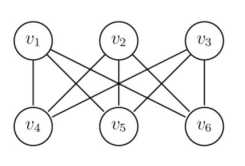
\includegraphics[scale=0.4]{32_2.png}
\end{figure}

У него $n=6, r = 9$. Если бы граф $K_{3,3}$ был планарным, то из равенства
$6 - 9 + q = 2$ получаем: $q=5$, поэтому $5 = q_3 + q_4 + \dots$

У графа K3,3 циклы минимальной длины могут иметь длину 4, циклов длины
5 нет (у двудольного графа циклы не могут иметь нечетную длину), могутеще быть циклы длины 6,
поэтому $5 = q_4 + q_6$ Решениями этого уравнения
являются пары: (0,5), (1,4), (2,3), (3,2), (4,1), (5,0).

Имеем также равенство: $2r = 18 = 4q_4 + 6q_6$. Ни одна из пар предыдущего
равенства не является решением этого уравнения.

Поэтому граф $K_{3,3}$ не является планарным.

Граф $K_{3,3}$ связан с теоремой о трех соседях и трех колодцах: нужно от
каждого из домов трех соседей к каждому из трех колодцев провести
дорожки, которые бы не пересекались. Так как граф $K_{3,3}$ не является
планарным, то это сделать невозможно.

\begin{theorem}
    \textbf{(Критерий Понтрягина -- Куратовского плоской реализуемости
графа)}

    Конечный граф $G$ является планарным тогда и только тогда, когда он не имеет
    подграфов, гомеоморфных $K_5$ или $K_{3,3}$.
\end{theorem}
  \section{Теорема об укладке графа в трехмерном пространстве.}

\begin{theorem}
    Любой конечный граф можно уложить в трёхмерном пространстве.
\end{theorem}

\begin{proof}
    Рассмотрим произвольный граф с $n$ вершинами и $r$ рёбрами.
    Проведем прямую, отметим на ней $n$ различных точек. Каждой из них
    сопоставим вершину графа. Через прямую проведем $r$ различных плоскостей,
    каждой плоскости сопоставим ребро графа. Каждому ребру $(u,v)$ сопоставим
    полуокружность, соединяющую вершины $u$ и $v$, и проходящую в плоскости,
    соответствующей данному ребру. Очевидно, что такие ребра не будут
    пересекаться во внутренних точках.
\end{proof}
  \section{Хроматическое число и хроматический индекс графа. Теорема о хроматическом числе графа в 
простейших случаях. Теорема о четырех красках. Найти хроматическое число графа. Ответ 
обосновать.}

\begin{definition}
    \textit{Раскраской графа (вершинной раскраской, правильной
    вершинной раскраской)} называется такое приписывание цветов вершинам
    графа, что смежным вершинам сопоставляются разные цвета.
\end{definition}

\begin{definition}
    Граф называется \textit{n-раскрашиваемым},
    раскраска графа, использующая n цветов.
\end{definition}

\begin{definition}
    Хроматическим числом графа $\chi(G)$ называется минимальное
    количество цветов в раскраске этого графа.
\end{definition}

\begin{theorem}
    Оценка хроматического числа графа в простейших случаях.
    \begin{enumerate}[left=0.0em, labelsep=1em, topsep=0.0em, itemsep=0pt, parsep=0.5em]
        \item $\chi(G)=1$ тогда и только тогда, когда граф не содержит ни одного ребра;
        \item $\chi(G)=2$ тогда и только тогда, когда $G$ -- двудольный граф, содержащий хотя бы одно ребро;
        \item если $G$ -- дерево, содержащее хотя бы одно ребро, то $\chi(G)=2$;
        \item если $K_n$ -- полный граф, то $\chi(K_n)=n$;
        \item если в графе есть полный подграф $K_s$, то $\chi(G) \geq s$.
    \end{enumerate}
\end{theorem}

\begin{proof}
    Оценка хроматического числа графа в простейших случаях.
    \begin{enumerate}[left=0.0em, labelsep=1em, topsep=0.0em, itemsep=0pt, parsep=0.5em]
        \item Если в графе нет рёбер, то всем вершинам можно приписать один цвет.
        \item Вершины из одной доли раскрашены в один цвет и не смежны по определению.
        Доли всего две, следовательно, $\chi(G)=2$.
        \item Дерево -- двудольный граф без циклов. Аналогично 2, $\chi(G)=2$.
        \item Так как все вершины графа смежные, то им необходимо сопоставить
        разные цвета.
        \item В полном графе на $n$ вершинах, можно выделить полный подграф
        $n-1$. $\chi({G}')=n-1$ для подграфа, $\chi(G)=n$ для самого графа. Тогда $n \geq n - 1$. 
    \end{enumerate}
\end{proof}

\newpage
Одной из основных теорем математики являются теорема о \textbf{четырёх красках}.
Очень долго она была гипотезой, но сейчас считается теоремой.

Пусть есть некоторая карта государств, при этом два государства называются
соседними, если они имеют общую границу.

\begin{theorem}
    Пусть каждое государство является односвязной областью, соседние
    государства имеют протяжённую границу. Тогда их можно раскрасить,
    используя не более 4 цветов так, чтобы соседние государства были
    раскрашены в разный цвет.

    Рассмотрим столицы этих государств. Им сопоставим вершины графа. Если
    страны являются соседними, то соединим вершины, соответствующие их
    столицам, рёбрами. Тогда теорему можно сформулировать следующим
    образом:
\end{theorem}

\begin{theorem}
    Хроматическое число планарного графа не больше четырех.
\end{theorem}

\begin{proof}
    Теорема была доказана в 1978 году с помощью ЭВМ и пока не имеет
    доказательства в традиционном понимании.
\end{proof}

\textbf{Алгоритм последовательной раскраски:}
\begin{enumerate}[left=0.0em, labelsep=1em, topsep=0.0em, itemsep=0pt, parsep=0.5em]
    \item Упорядочиваем вершины графа $G$ в порядке невозрастания степеней --
    от вершин максимальной степени к минимальной.
    Получаем последовательность L.
    \item Полагаем цвет окраски p=1.
    \item Если список L пуст, то останавливаемся. Если нет, то переходим к шагу
    4.
    \item Окрашиваем в цвет p первую вершину из списка L и все вершины,
    которые не смежны с вершинами, уже окрашенными в цвет p, рассмотрение
    этих вершин производим в порядке, в котором они находятся в
    последовательности L. После того, как вершина получила цвет, удаляем ее из
    списка. После рассмотрения всех вершин последовательности р:=p+1.
    Переходим к шагу 3.
\end{enumerate}

\newpage
Пример раскраски на графе.
\begin{figure}[h]
    \centering
    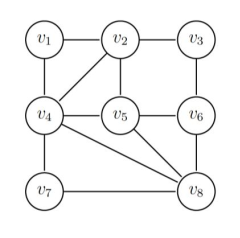
\includegraphics[scale=0.5]{34_1.png}
\end{figure}
\begin{figure}[h]
    \centering
    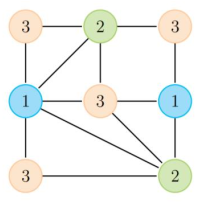
\includegraphics[scale=0.5]{34_2.png}
\end{figure}

Очевидно, что раскраска оптимальна, так как в графе есть подграф $K_3$,
и следовательно, $\chi(G) \geq 3$.

\begin{definition}
    \textit{Рёберной раскраской графа} называется приписывание рёбрам
    цветов так, чтобы рёбра, имеющие общую вершину, были раскрашены в
    разные цвета.
\end{definition}

\begin{definition}
    \textit{Хроматическим индексом графа} называется минимальное
    количество цветов в реберной раскраске графа.
\end{definition}

\begin{theorem}
    Хроматический индекс графа равен $\delta$ или $\delta+1$, где
    \begin{align*}
        \delta = \max \delta(v), v \in V.
    \end{align*}
\end{theorem}
  \section{Эвристический алгоритм нахождения хроматического числа графа. Применить для указанного 
графа.}


  \section{Хроматический многочлен, его свойства и методы нахождения. Найти хроматический многочлен 
графа.}

\begin{definition}
    Пусть $G=(V,E)$ -- некоторый граф и $t$ -- заданное число цветов.
    Число способов правильной раскраски графа $G$ с возможностью
    использования $t$ цветов называется его \textit{хроматическим многочленом} и
    обозначается $P(G,t)$.
\end{definition}

Рассмотрим хроматические многочлены для некоторых графов.
\begin{enumerate}[left=0.0em, labelsep=1em, topsep=0.0em, itemsep=0pt, parsep=0.5em]
    \item $P(G,t)$ графа из одной вершины без ребер равен $t$.
    \item $P(G,t)$ графа из двух вершин без ребер равен $t^2$.
    \item $P(G,t)$ графа из $n$ вершин без ребер (нульграфа) равен $t^n$.
    \item $P(G,t)$ полного $n$-вершинного графа $K_n$ равен
    
    $t(t-1)(t-2) \dots (t-(n-1))$.
    \item $P(G,t)$ дерева с $n$ вершинами равен $t(t-1)^{n-1}$.
    \item $P(G,t)$ графа из $n$ вершин, который является цепью равен $t(t-1)^{n-1}$.
    \item $P(G,t)$ графа из $n$ вершин, который является циклом, равен
    
    $(t-1)^n +(-1)^n(t-1)$.
\end{enumerate}


\textbf{Теоремы Зыкова}

Две теоремы, рассмотренные ниже, позволяют находить хроматический
многочлен графа.

Рассмотрим три операции на графах: удаление ребра, добавление ребра и
стягивание двух несмежных вершин.

В первой операции у графа из множества ребер удаляется выбранное ребро
$(u, v)$, граф в этом случае обозначается $G \setminus \set{(u, v)}$.

Во второй операции добавляется ребро $(u, v)$, которого не было, граф в этом
случае обозначается $G \cup \set{(u, v)}$.

В третьей операции две вершины $u, v$ отождествляются, вместо них берется
новая вершина, эта вершина в новом графе смежна всем вершинам,
которым смежна хотя бы одна из вершин $u, v$, граф в этом случае
обозначается $G/(uv)$.

Хроматический многочлен можно находить с помощью двух теорем.

\begin{theorem}
    \textbf{(Зыкова 1)}. Пусть $(u, v)$ -- ребро графа $G$, $t$ -- количество цветов,
    используемых при раскраске. Тогда
    \begin{align*}
        P(G,t) + P(G/(uv), t) = P(G \setminus \set{(u,v)},t).
    \end{align*}
\end{theorem}

\begin{proof}
    Выражение $P(G \setminus \set{(u,v)},t)$ в правой части равенства -- это
    число возможных правильных раскрасок графа $G$ c удаленным ребром
    $(u,v)$, поэтому в нем вершины u и v могут иметь как одинаковый, так и
    разные цвета.
    
    В левой части равенства слагаемое $P(G,t)$ -- это число различных
    правильных раскрасок графа $G$, в которых смежные вершины u и v имеют
    разные цвета, в слагаемом $P(G/(uv), t)$ вершины $u$ и $v$ стянуты в одну,
    поэтому имеют один цвет. Поэтому равенство справедливо.
    
    Если равенство записать в виде $P(G,t) = P(G \setminus \set{(u,v)},t) - P(G/(uv), t)$,
    
    то его можно использовать для нахождения хроматического многочлена,
    каждый раз производя операции удаления ребра и стягивания
    
    Этот алгоритм называют \textit{редукцией по нуль-графам} или \textit{алгоритмом
    Зыкова}.
\end{proof}

\begin{theorem}
    \textbf{(Зыкова 2)}. Пусть $u, v$ -- несмежные вершины графа $G$. Тогда
    \begin{align*}
        P(G,t) = P(G \cup \set{(u,v)},t) + P(G/(uv), t)
    \end{align*}
\end{theorem}

Применение этой теоремы для нахождения хроматического многочлена
называется редукцией по полным графам.

%TODO: ПРИМЕР

\newpage
Пусть хроматический многочлен графа $G$ имеет вид:
\begin{align*}
    P(G,t) = a_nt^n + a_{n-1}t^{n-1}+ \dots +a_1t+a_0.
\end{align*}

Справедливы следующие свойства хроматического многочлена:
\begin{enumerate}[left=0.0em, labelsep=1em, topsep=0.0em, itemsep=0pt, parsep=0.5em]
    \item Свободный член хроматического многочлена $a_0$ равен нулю.
    \item Старший член хроматического многочлена $a_n$ равен 1.
    \item Степень хроматического многочлена равна числу вершин в графе.
    \item Пусть $v$ -- висячая вершина графа $G$, пусть $G_1$ -- граф, полученный из
    графа $G$ удалением этой вершины и инцидентного ей ребра. Тогда
    $P(G,t) = (t-1) P(G_1,t)$
    \item Пусть $v$ -- вершина графа $G$ степени два, смежная с двумя вершинами $u$
    и $w$, которые, в свою очередь, смежны друг с другом (то есть три эти
    вершины образуют граф $K_3$). Пусть $G_1$ -- граф, полученный из графа $G$
    удалением этой вершины и двух инцидентных ей ребер. Тогда
    $P(G,t) = (t-2) P(G_1,t)$
    \item Пусть $G_1, G_2, \dots, G_s$ -- компоненты связности графа $G$.
    
    Тогда $P(G,t) = \prod_{i=1}^{s}(G_i, t)$
\end{enumerate}

\end{document}